\chapter{Text Representation}\label{ch:text-representation}

\section{Overview}\label{sec:overview_text_representation}
The key question in text processing and \gls{nlp} is how to encode text into numbers so that computers can understand them.
The process is also known as \emph{Vectorization} \cite{word2vec2} and there are two main approaches to vectorize text.\\
The first and more traditional approach is to encode word or \gls{token} occurrence counts.
A more modern approach is to train Artificial Neural Networks (\gls{ann}) to get text embeddings that also incorporate syntax and semantics.
In the next subsections, I will explain these encoding techniques as they form the foundation for most of the subsequent chapters.


\section{Definitions}\label{sec:definitions}
In \gls{nlp}, the terms \gls{corpus}, \gls{vocabulary} and \gls{document} are often interpreted differently which requires clarification.
In this thesis, a \gls{document} is defined as text that might contain multiple sentences such as a news article in the data described above.
All news articles in the entire data set constitute the \gls{corpus} which refers to a collection of documents.
All unique words in a \gls{corpus} represent the \gls{vocabulary}.
A \gls{document_term_matrix} is a tabular data structure where rows represent references to documents and columns represent the unique terms of a vocabulary.
Such terms or \glspl{token} can either be words or sub-words and in a \gls{document_term_matrix} represent its features.
The data entries in the \gls{document_term_matrix} are the feature values and show if or how often the term appears in the respective document.

A simplified example can be seen in Fig.\ref{fig:sample_docs} and in Fig.\ref{fig:document_term_matrix}:

\begin{figure}[H]
    \centering
    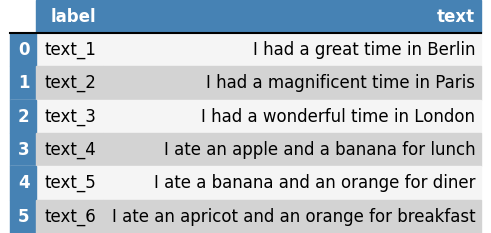
\includegraphics[keepaspectratio=true,scale=0.6]{Assets/topic_model_text}
    \caption{Sample Documents}
    \label{fig:sample_docs}
\end{figure}

The text in each row is a \gls{document} though in this example only contains one sentence each and
the \gls{corpus} here constitutes all six \glspl{document}.


\begin{figure}[H]
    \centering
    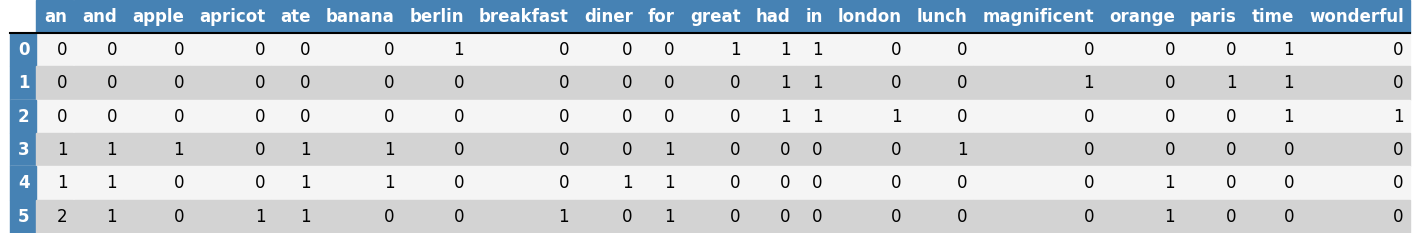
\includegraphics[width=1.0\textwidth]{Assets/topic_model_count_vector}
    \caption{Document Term Matrix}
    \label{fig:document_term_matrix}
\end{figure}

The \gls{document_term_matrix} is shown in Fig.\ref{fig:document_term_matrix} where the header row represents the \gls{vocabulary}.
The data entries in the table are the counts for each \gls{vocabulary} term in each \gls{document}.


\section{Traditional Methods}\label{sec:traditional-methods}

\subsection{One-Hot-Encoding}\label{subsec:one-hot-encoding}
Each \gls{document} in the Fig.\ref{fig:sample_docs} can be represented by the respective row in Fig.\ref{fig:document_term_matrix} when interpreted as a vector.
$$\vec{document_0} = [\;0\;0\;0\;0\;0\;0\;1\;0\;0\;0\;1\;1\;1\;0\;0\;0\;0\;0\;1\;0\;]$$
If such vectors only contain binary ones and zeros, i.e. if they do not count word occurrences but only indicate if a word is present or not, such vectors are called One-Hot encoded vectors.


\subsection{Bag-of-Words}\label{subsec:bag-of-words}
The \gls{document_term_matrix} shown in Fig.\ref{fig:document_term_matrix} also contains word counts as can be seen from the \gls{document} in the last row:
$$\vec{document_5} = [\;2\;1\;0\;1\;1\;0\;0\;1\;0\;1\;0\;0\;0\;0\;0\;0\;1\;0\;0\;0\;]$$
Such vectors are known as Bag-of-Word vectors as they account for the frequency of a word in a \gls{document}.

\subsection{Document Similarities}\label{subsec:document-similarities}
After vectorization, it is possible to calculate similarities between sentences mathematically.
One common way to do that is to calculate the cosine similarity of the desired vectors which is the cosine of the angles between the two vectors \cite{CosineSimilarity}:

\begin{equation}
cosine\;similarity\,{_{ab}} = \frac{\vec{a} \cdot  \vec{b}^{\;T}}{\lvert{\vec{a}}\rvert \cdot \lvert{\vec{b}}\rvert}\label{eq:cossim1}
\end{equation}

For instance: The cosine similarity between document 0 and document 1 of the Sample Documents (Fig.\ref{fig:sample_docs}) is calculated by:

$$ cosine\;similarity\,{_{01}} = \frac{\vec{document0} \cdot  \vec{document1}^{\,T}}{\lvert{\vec{document0}}\rvert \cdot \lvert{\vec{document1}}\rvert} = 0.60 $$

The high cosine similarity of 0.60 is also attributed to the fact that both documents contain the same words
$$ [\;I,\;had,\;a,\;time,\;in\;] $$
some of which are considered \gls{stop_words} that do not carry much semantic information.

\subsection{Feature Dimension Reduction}\label{subsec:techniques-to-reduce-vocabulary}
Usually a \gls{document} contains far fewer terms than a \gls{vocabulary} which results in sparse vectors where many features have zero values.
Sparse vectors not only increase the computational complexity and the risk to overfit a Machine Learning model, but also are a sign that some
important information in the data is missing \cite{ProblemsWithSparseVectors}.
For this reason, it is common practice to reduce the \gls{vocabulary} and so the vector and feature dimension.

\subsubsection{Remove Stop Words}\label{subsubsec:remove-stop-words}
\gls{stop_words} include articles, conjunctions, prepositions, pronouns and very common verbs such as \emph{is}.
They appear in most \glspl{document} and thus do not contribute to distinguish them.
Beside commonly known \gls{stop_words} in a \gls{corpus}, there might be additional domain-specific \gls{stop_words} such as the word for the currency unit \emph{Euro} in finance-related \glspl{document}.

\subsubsection{Remove Function Words}\label{subsubsec:remove-function-words}
\gls{nlp} differentiates between \gls{content_words} and \gls{function_words}.
\gls{function_words} help to construct the grammatical relationships in a sentence whereas \gls{content_words} serve to carry their semantic meaning.
In Topic Modelling, the target is to extract semantics. Thus, \gls{function_words} are less relevant and can be removed.

\subsubsection{Reduce words to their Lemmas and Stems}\label{subsubsec:word-lemmas}
Words appear in many different inflectional forms such as verb tenses (past, present and future) and pluralizations.
\gls{lemmatization} is the process to convert all such forms to the lemma or root of the word \cite{Lemmatization}.
This process removes some contextual information but usually well preserves the semantic meaning of the text.
\gls{stemming} reduces a word to its word stem by clipping off some suffix chars.
Contrary to \gls{lemmatization}, this process can change the semantic meaning of the word (for instance: \emph{fisher}\textrightarrow \emph{fish}) and thus must be
applied carefully.
Nevertheless, both methods drastically reduce the size of the \gls{vocabulary}.

\subsubsection{Others}\label{subsubsec:others}
Other methods to reduce the \gls{vocabulary} include the removal of non-words such as punctuation chars and numbers from the text.
If nouns in a specific domain carry proportionally more information than other words, it might be beneficial to remove all non-noun words.


\subsection{TF-IDF}\label{subsec:tf-idf}
It is known from Information Theory that low probability terms carry much more information than high probability terms \cite{EntropyInformationTheory}.
Low probability terms are those words that appear very seldom in a \gls{corpus} or in the \glspl{document} that were used to train commonly used \glspl{llm}.
If such low probability words appear much more frequently in a certain \gls{document} than in the related \gls{corpus}, this might be an indication
that this word is important to understand the context of the particular \gls{document}.
This is the concept of \gls{tfidf}:

\begin{gather}\label{eq:tfidf}
    \emph{TF-IDF} = TF * IDF
\notag \\ \notag \\
    \emph{TF} = \frac {\textrm{number of times the \textbf{term} appears in the document} }{ \textrm{total number of terms in the document}}
\notag \\ \notag \\
    \emph{IDF} = log\; (\frac {\textrm{number of documents in the corpus}} {\textrm{number of documents in the corpus containing the \textbf{term}}})
\notag \\ \notag \\
\end{gather}

The Term Frequency (TF) is the frequency a target word appears in a given \gls{document}.
In a Bag-of-Word approach (Sec.\ref{subsec:bag-of-words}), this number would go into the \gls{document_term_matrix}, but
in \gls{tfidf}, it is first multiplied by the Inverse Document Frequency (IDF).
The IDF is the logarithm of the number of all \glspl{document} divided by the number of those \glspl{document}
that contain the target word.
If the frequency of the target word in all \gls{document} is low, then the IDF will be high and this will increase the weight of
the target word in the \gls{document_term_matrix}.
This can be seen from the \gls{document_term_matrix} in Fig.\ref{fig:document_term_matrix_tfidf} when \gls{tfidf} vectorization was used:

\begin{figure}[H]
    \centering
    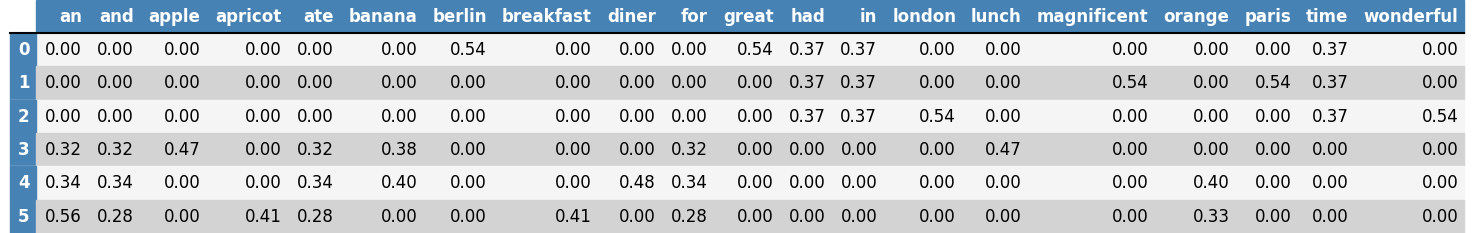
\includegraphics[width=1.0\textwidth]{Assets/topic_model_tfidf_vector}
    \caption{Document Term Matrix with TF-IDF}
    \label{fig:document_term_matrix_tfidf}
\end{figure}

Words that appear only once in all \glspl{document} (for instance the word \emph{apple}) have a higher weight in the \gls{tfidf} \gls{document_term_matrix} than words
that appear very often (for instance the word \emph{ate}).

%%%%%%%%%%%%%%%%%%%%%%%%%%%%%%%%%%%%%%%%%%%%%%%%%%%% EMBEDDINGS
\section{Word Embeddings\protect\footnote{This section was mainly taken from \cite{LfdTalk15}}}\label{sec:word-embeddings}


\subsection{Static Word Vectors}\label{subsec:static-word-vectors}

As explained in section \ref{subsec:one-hot-encoding}, words can be represented as one-hot encodings as also shown in the example in Fig.\ref{fig:onehot}.

\begin{figure}[H]
	\centering
	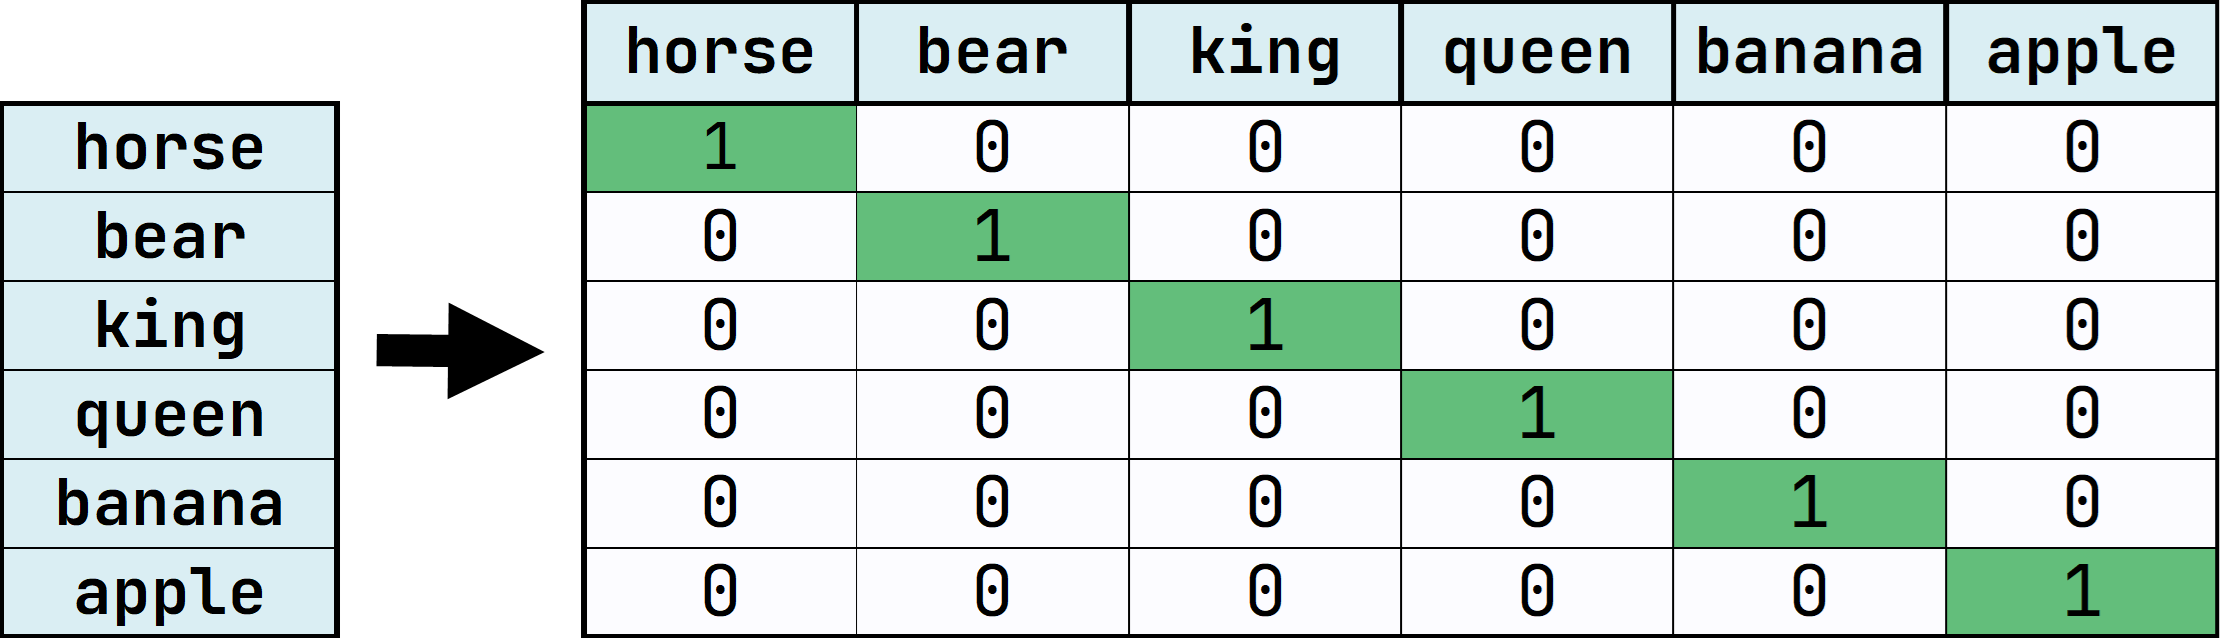
\includegraphics[width=0.7\textwidth]{Assets/onehot}
	\caption{One-Hot example}
	\label{fig:onehot}
\end{figure}

The first disadvantage of this approach is the computational inefficiency as each word in our simple example in Fig.\ref{fig:onehot} would require a sparse six-column vector with five 0's and only one 1.
The second disadvantage is that this approach does not encode syntactical or semantic word similarities as similar words would have different and unrelated vector representations.

\subsubsection{Manually crafted features}
To encode syntactical or semantic word commonalities, one could think about word characteristics or attributes and manually encode the magnitude of those attributes for each word as shown in Fig.\ref{fig:wordfeaturesmanually}.
A \emph{horse} is an \emph{animal}, one \emph{can ride it}, it has \emph{four legs} and is usually \emph{peaceful}.\\
This is very similar to the \gls{vocabulary} in the \gls{tfidf} and \emph{Bag-of-Word} approach outlined in Section \ref{subsec:tf-idf}, but differes from
it in that the features here do not represent actual words but contextual concepts.
The feature \emph{animal} only has values in its respective vector position, not when the \emph{word} \emph{animal} itself appears, but only when the \emph{contextual concept} of an \emph{animal} appears.

\begin{figure}[H]
	\centering
	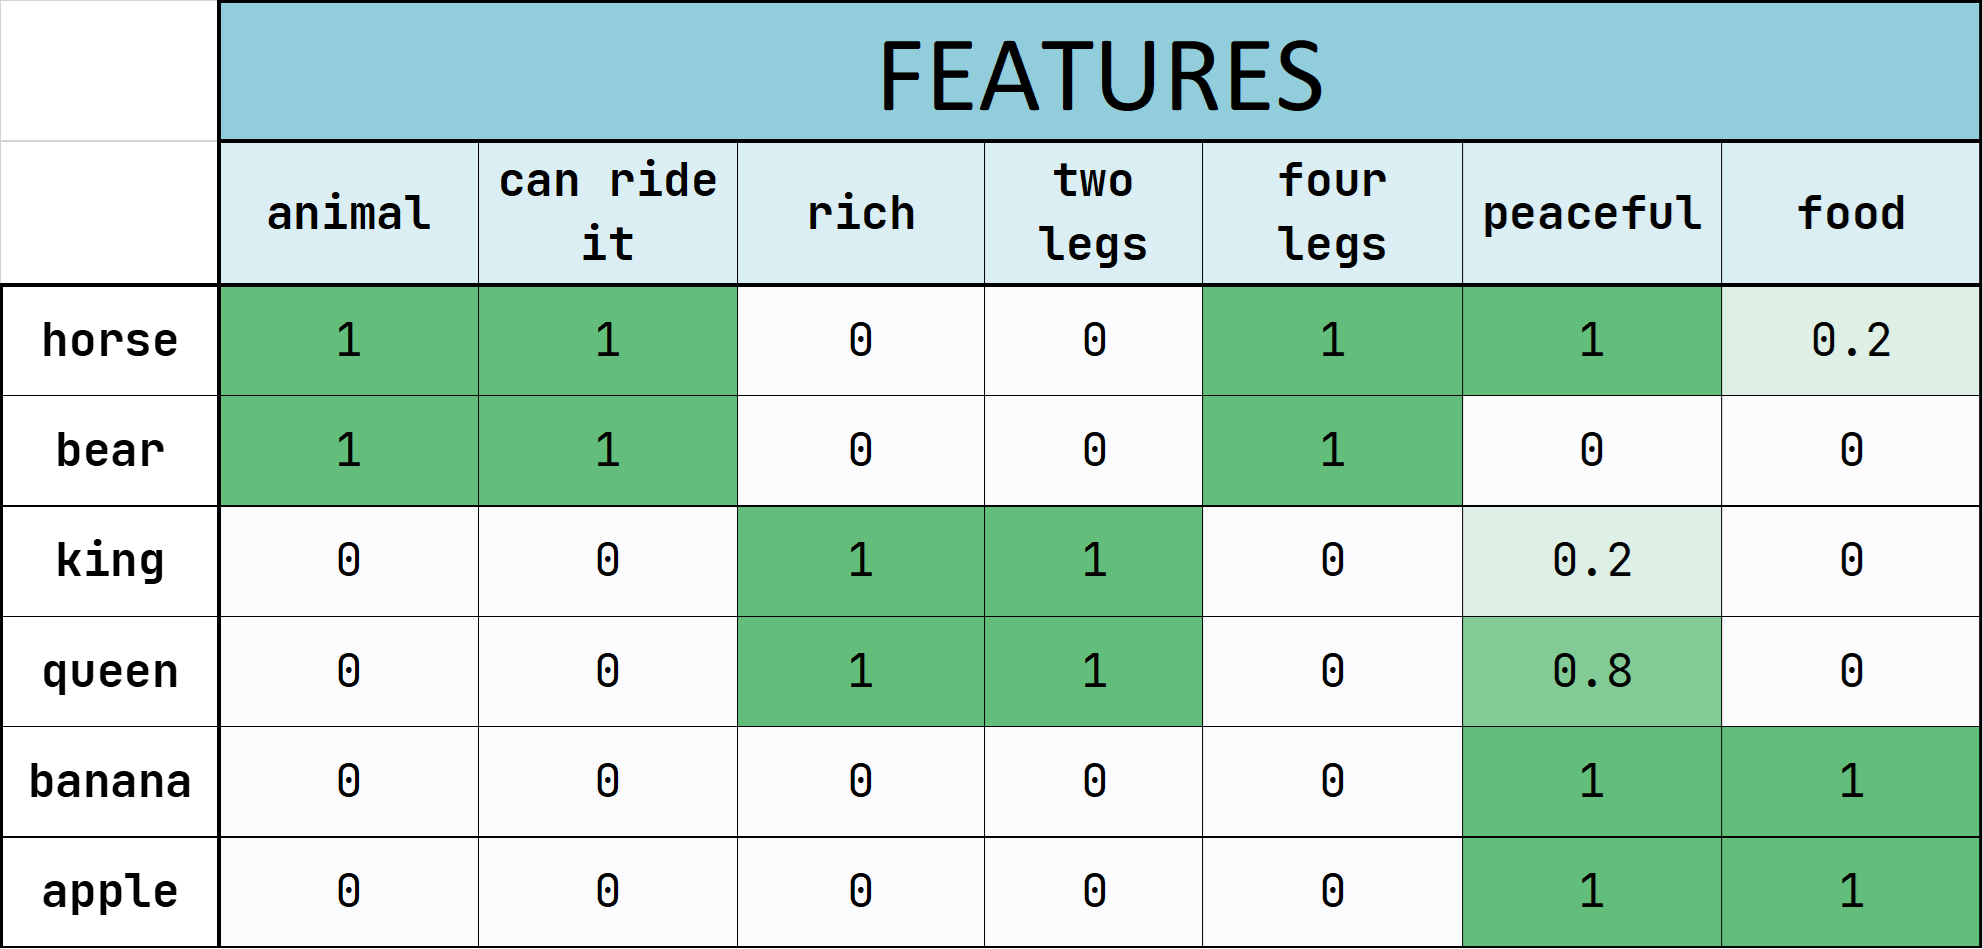
\includegraphics[width=0.7\textwidth]{Assets/wordfeaturesmanually}
	\caption{Manually Crafted Features}
	\label{fig:wordfeaturesmanually}
\end{figure}

The word \emph{horse} would then be represented as a vector of values for each of these handcrafted features (Fig.\ref{fig:horsevector}):

\begin{figure}[H]
	\centering
	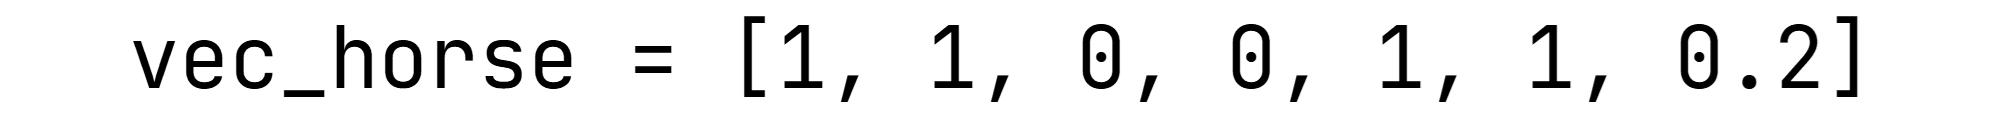
\includegraphics[width=0.7\textwidth]{Assets/horsevector}
	\caption{Word vector for the word \emph{horse}}
	\label{fig:horsevector}
\end{figure}

This approach ensures that related words are represented similarly as their values in the respective vector position are close to each other.
Such similarities can also be calculated numerically by applying the cosine similarity method, see Equation \ref{eq:cossim1}.
The cosine similarities between each pair of words in Figure \ref{fig:wordfeaturesmanually} are depicted in Fig.\ref{fig:cossimvalues}.

\begin{figure}[H]
	\centering
	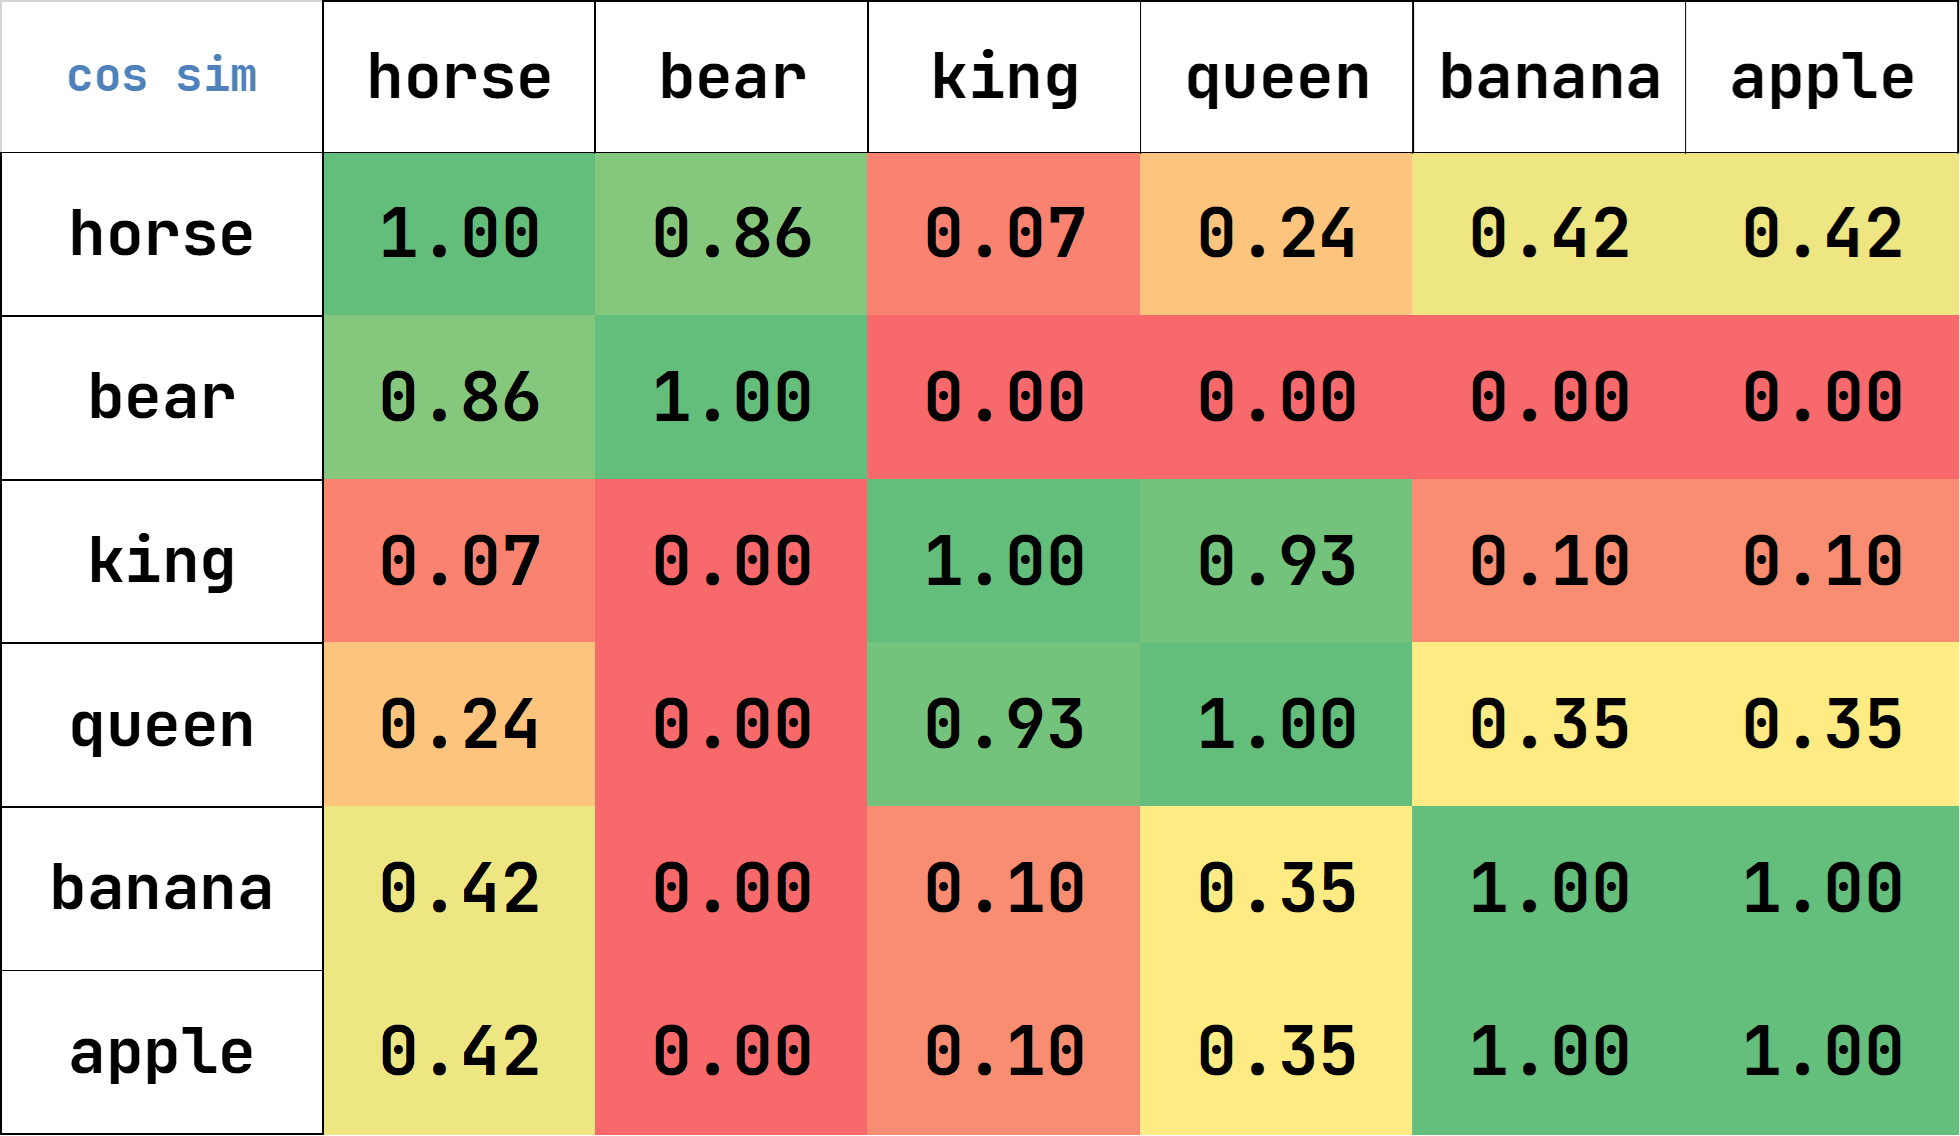
\includegraphics[width=0.6\textwidth]{Assets/cossimvalues}
	\caption{Exemplary Cosine Similarity Matrix based on Fig.\ref{fig:wordfeaturesmanually}.}
	\label{fig:cossimvalues}
\end{figure}

The cosine similarity for the word pair \emph{horse} and \emph{apple}, for instance, yields a value of 0.42.
For the word pair \emph{apple} and \emph{banana} however, this value is 1.0, owing to the fact that both are fruits and in our simple example have the same feature values at each index position of their word vector.

\subsubsection{Learned features}
Manually crafting feature values for every word in a vocabulary is cumbersome at best.
Better than crafting features by hand is to have a machine learning model to learn these features and feature values.
This is the \emph{word2vec} approach Mikolov et al. proposed in their seminal papers in 2013 \cite{word2vec1,word2vec2}.
A shallow, two-layer \gls{ann} (Fig.\ref{fig:featureslearned}) is trained with sentences that contain a masked word to be predicted (target or dependent variable) based on its non-masked adjacent words (input or independent variables) in that sentence.

\begin{figure}[H]
	\centering
	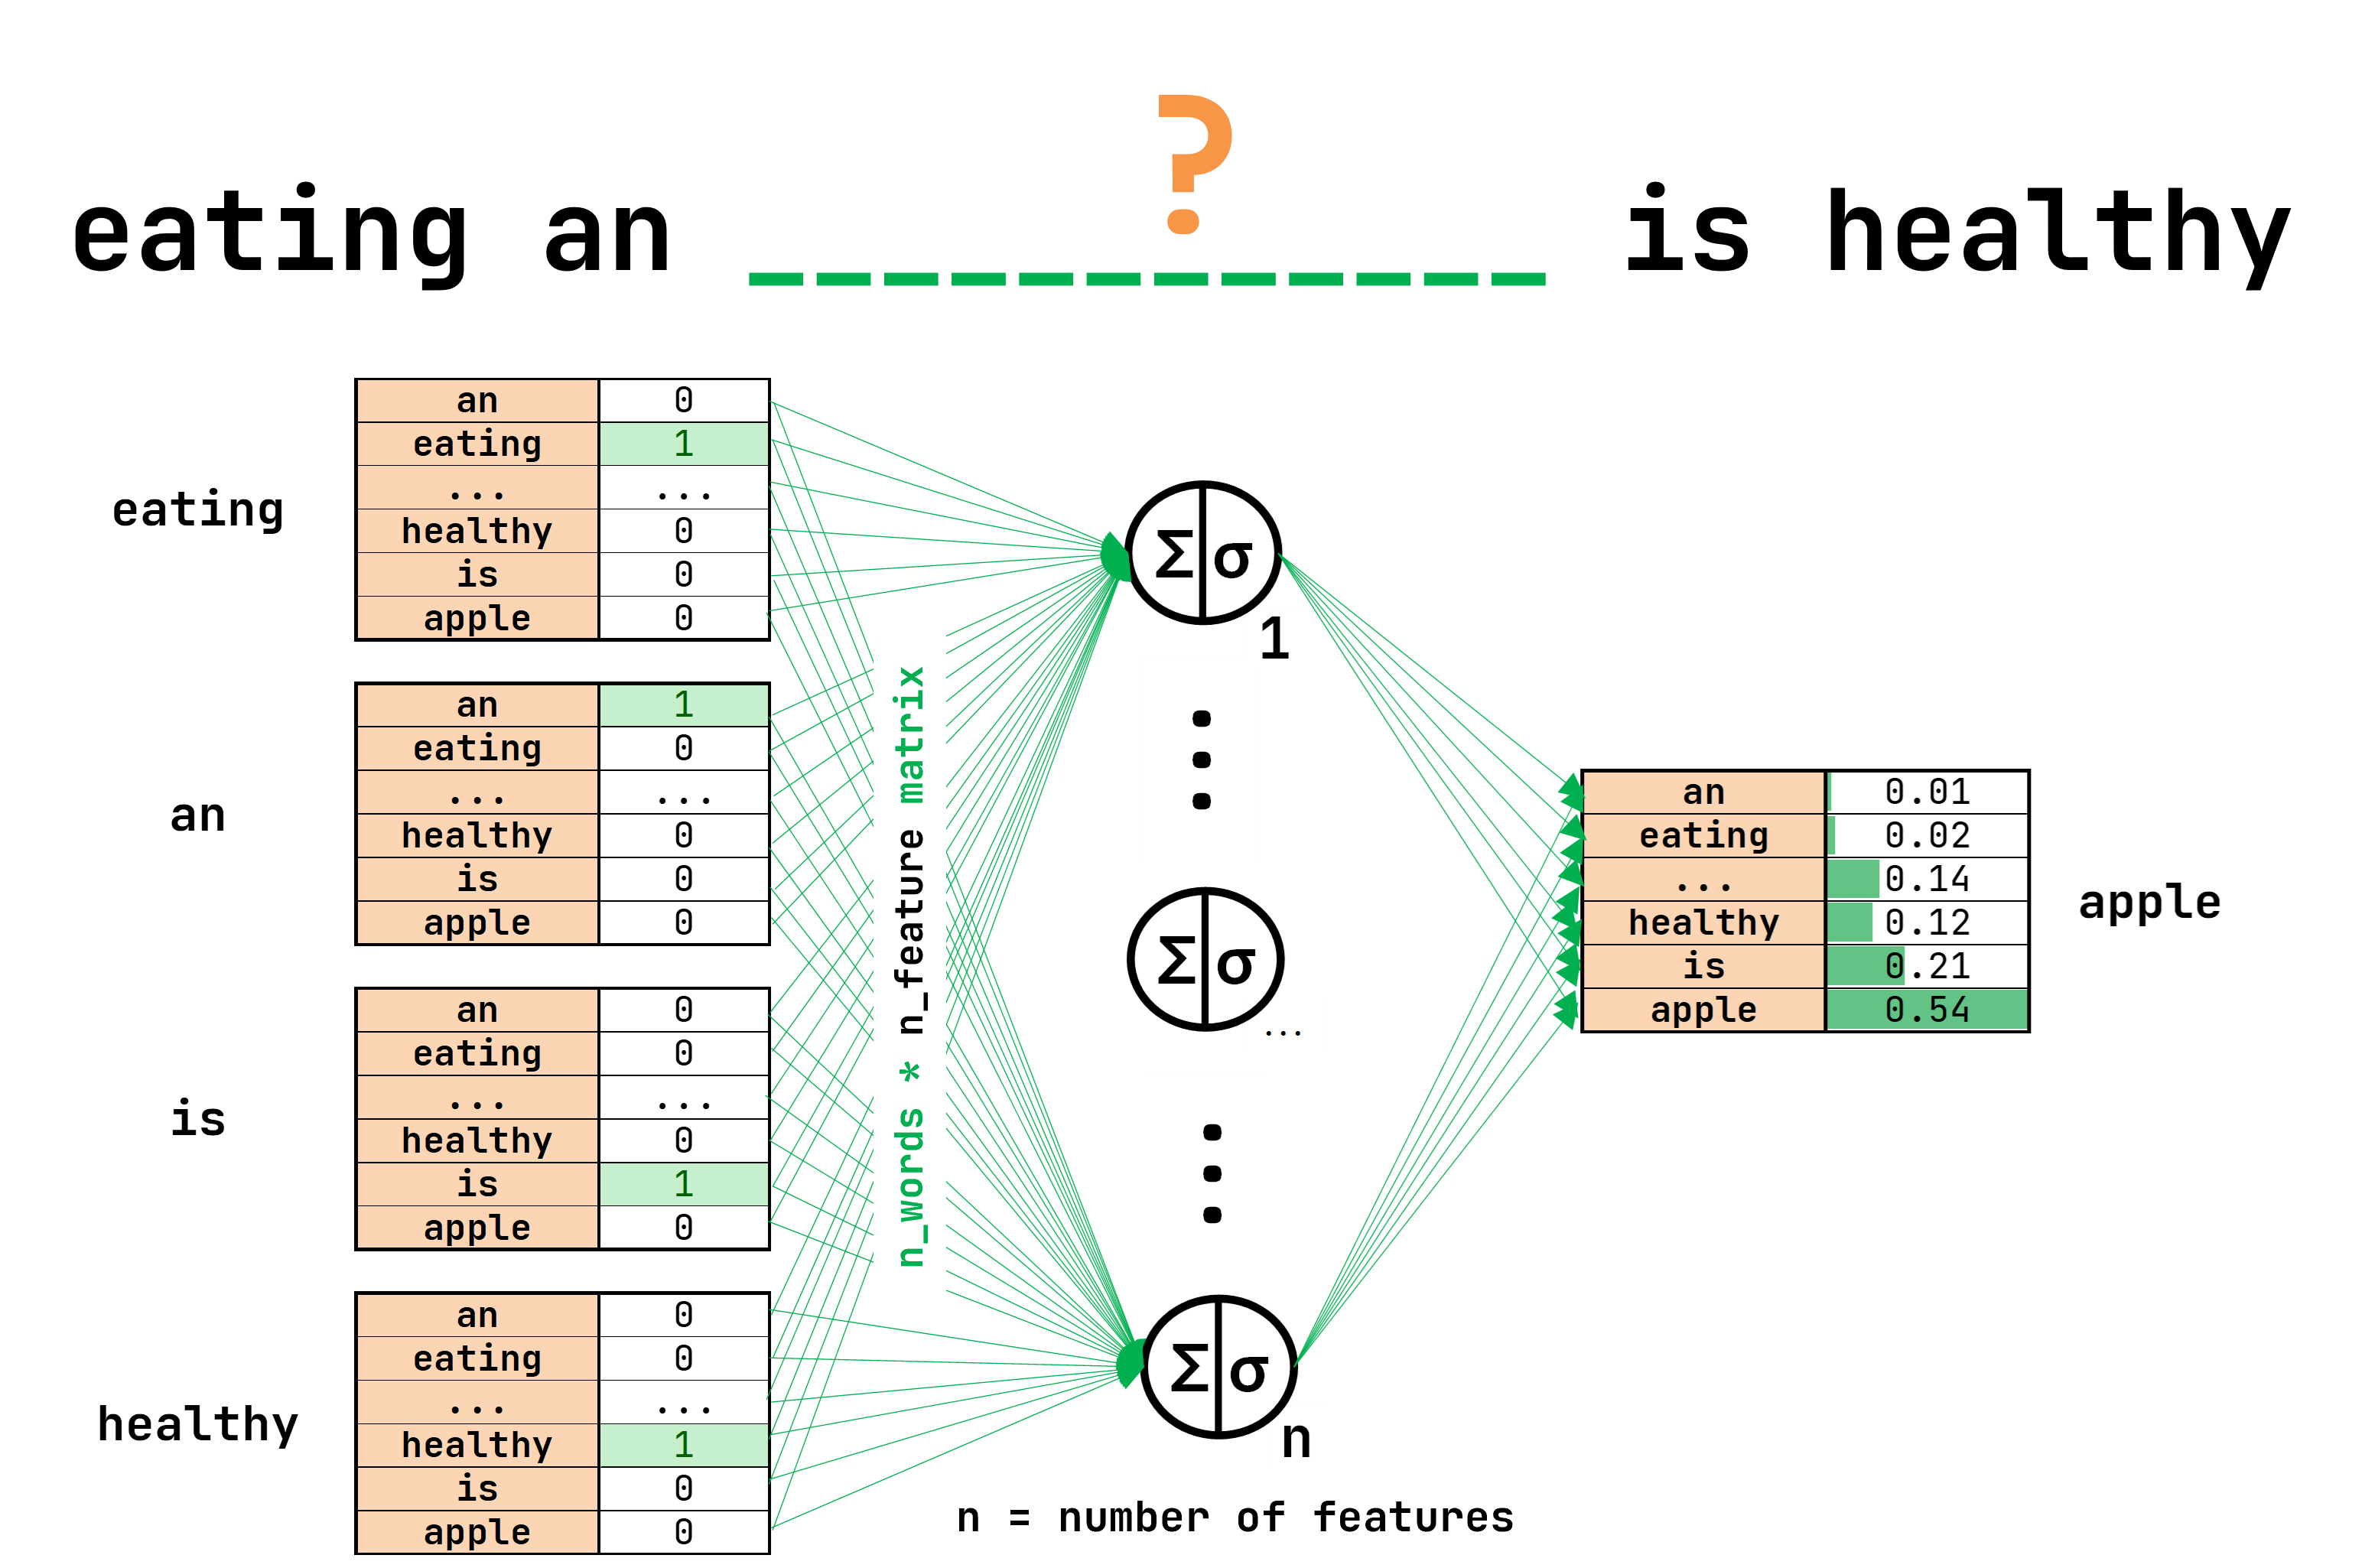
\includegraphics[width=0.6\textwidth]{Assets/featureslearned}
	\caption{word2vec: Masked words learned by a shallow, two-layer \gls{ann}.}
	\label{fig:featureslearned}
\end{figure}

The number of learned features depends on the number of neurons in the middle layer and the learned weights represent the respective feature values.
The learned features do not have names as before (like \emph{animal}, \emph{rich}, \emph{food}, etc.) and thus cannot be interpreted semantically by humans (easily) (Fig.\ref{fig:featvalueslearned}).

\begin{figure}[H]
	\centering
	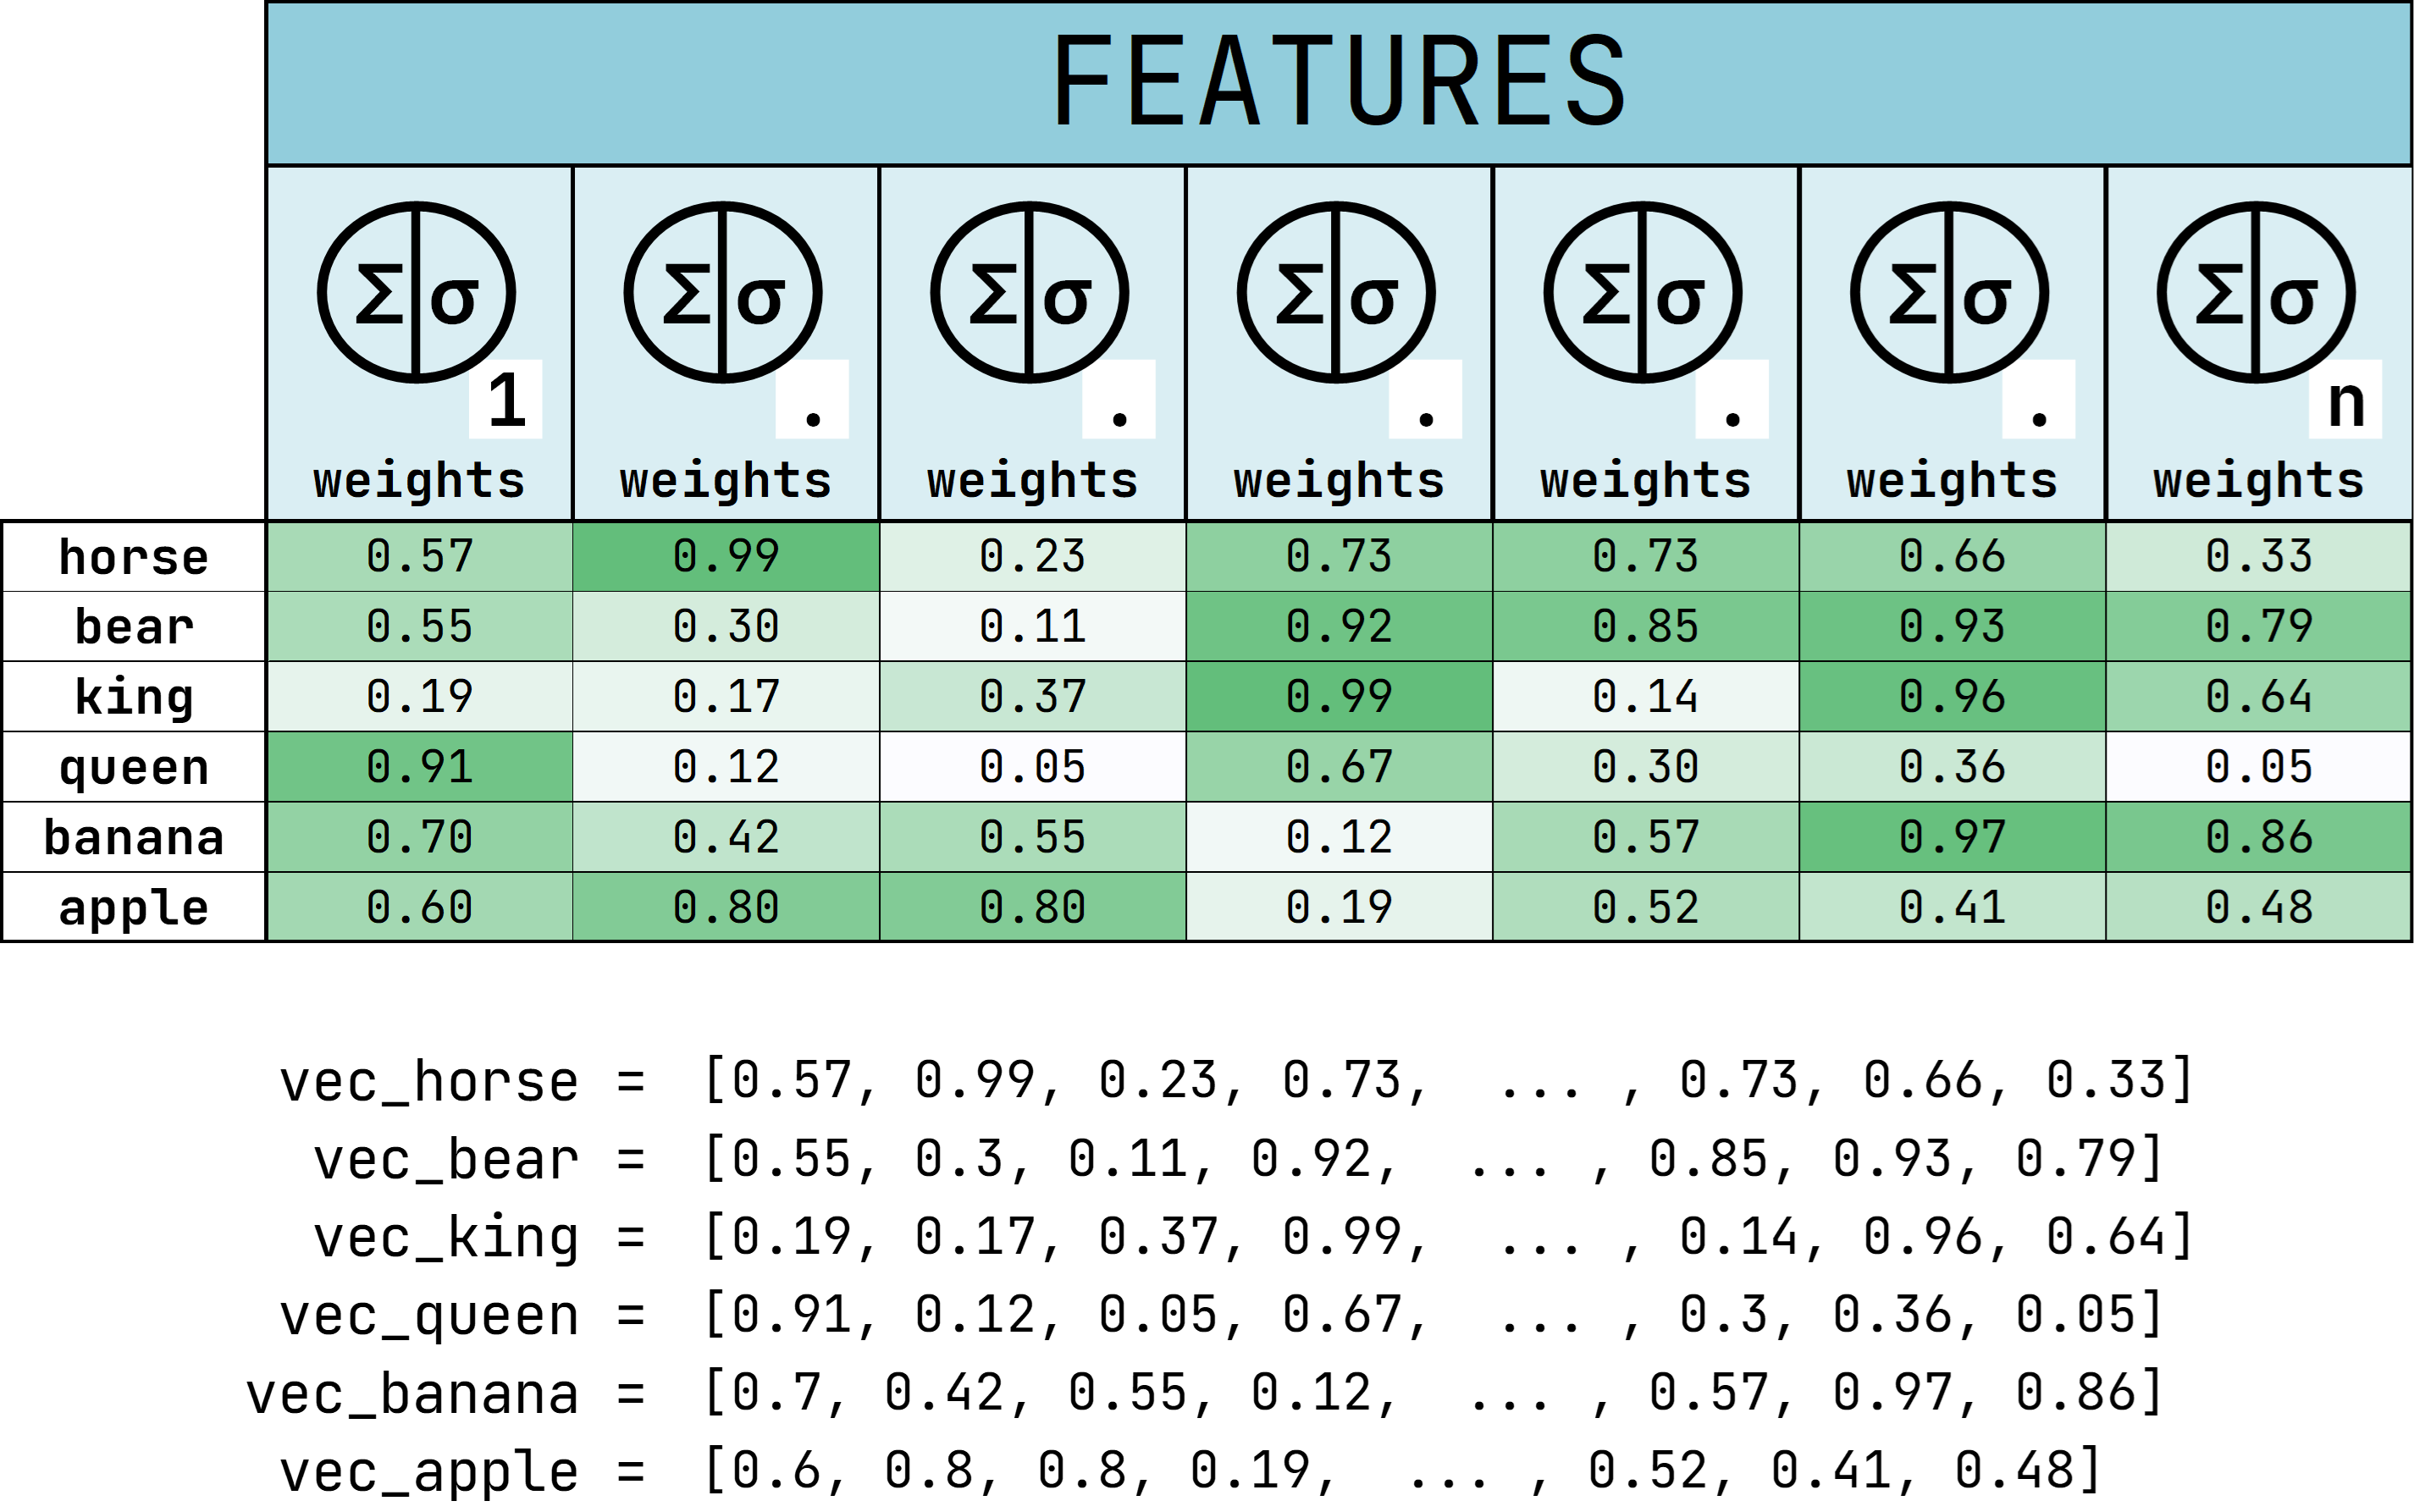
\includegraphics[width=0.8\textwidth]{Assets/featvalueslearned}
	\caption{The learned parameters/weights represent the feature values.}
	\label{fig:featvalueslearned}
\end{figure}

\subsubsection{The problem with static word embeddings}
The learned word vectors are also known as word embeddings and work well for tasks such as measuring similarities between individual words.
But they often fail when the scope goes beyond just words towards the semantic meaning of whole sentences.
A sentence is simply not just a chain of individual and independent words, but a construct containing interdependencies.

One of these word-wise interdependencies are homophones, i.e. words that are spelt the same but have different meanings.
The meaning of the word \emph{bank} in the sentence \emph{he withdraws money from his bank} is strongly affected by the surrounding words \emph{withdraws} and \emph{money} as they clearly suggest that \emph{bank} in that sentence refers to a financial institution.
In contrast, the meaning of the same word \emph{bank} in the sentence \emph{he was fishing in the river from a sand bank} is strongly affected by the words \emph{river} and \emph{sand} (Fig.\ref{fig:interdepend}).

\begin{figure}[H]
	\centering
	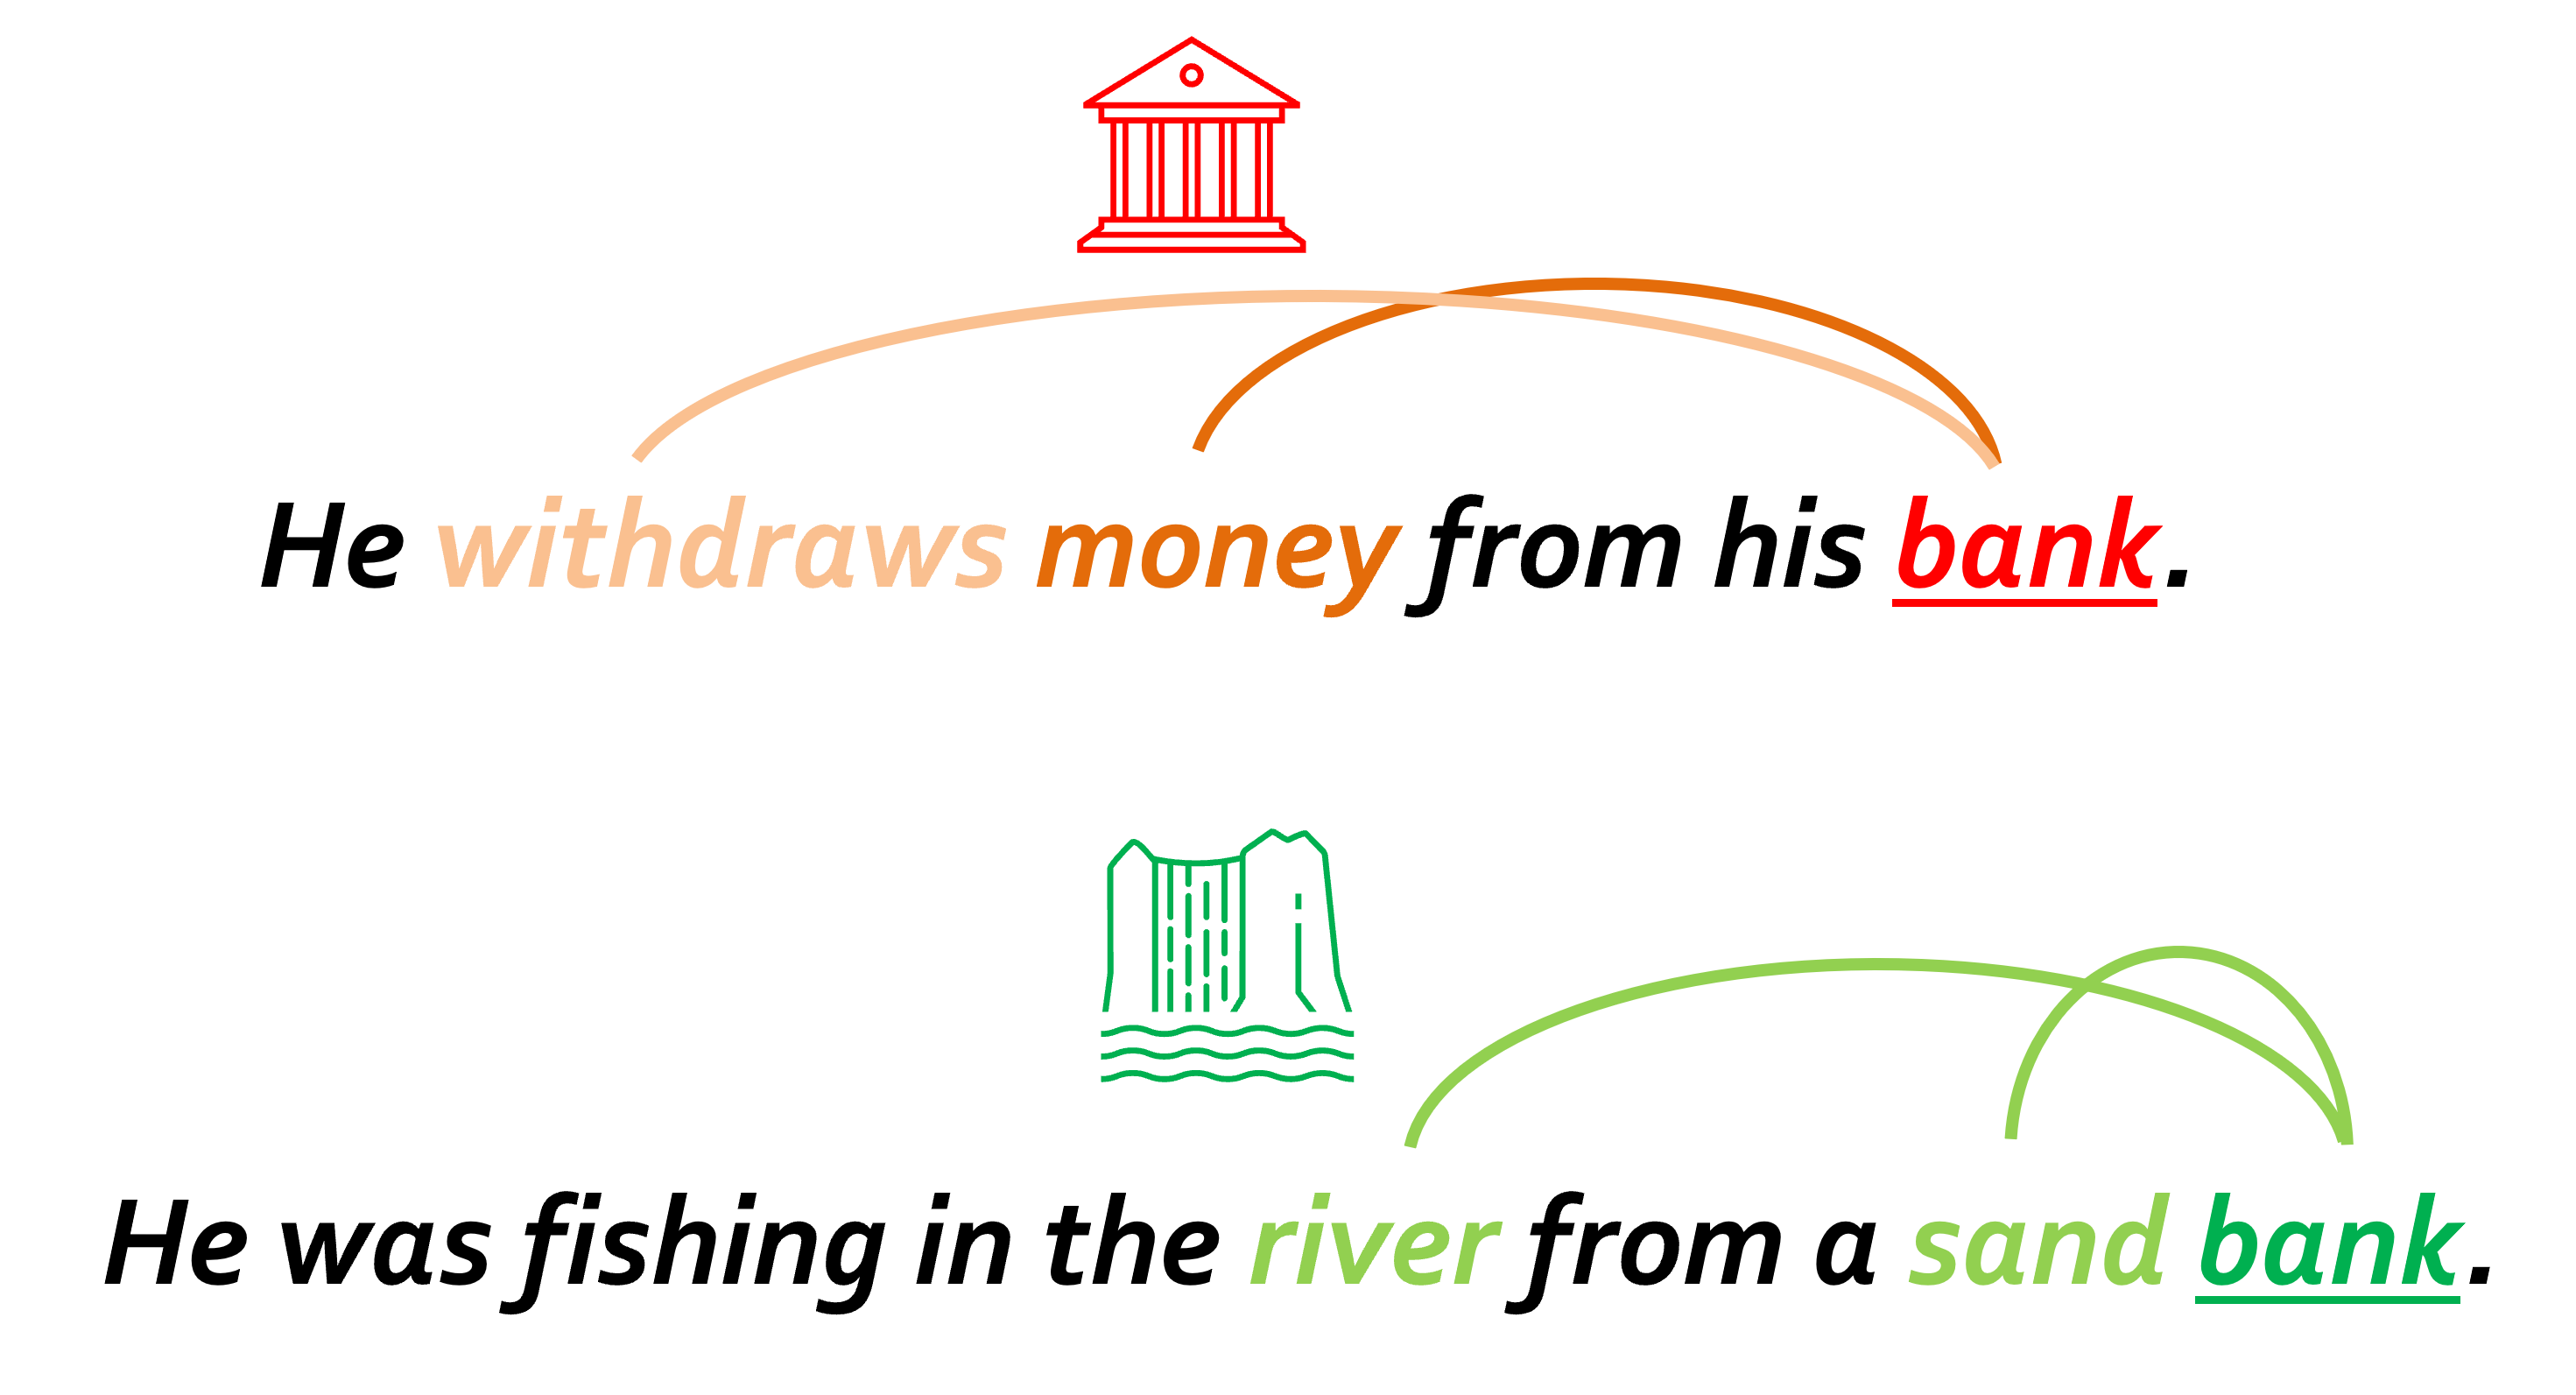
\includegraphics[width=0.7\textwidth]{Assets/interdepend}
	\caption{Homophone \emph{bank} dependent on its context}
	\label{fig:interdepend}
\end{figure}

When humans read these sentences, they derive the meaning of the word \emph{bank} by paying \emph{attention} to these adjacent words \cite{humanattention}.

There are more interdependencies in sentences than homophones, but in general it can be said that the meaning of a word depends on its respective context.
Word embeddings such as word2vec \cite{word2vec1,word2vec2} are static in the sense that they treat equal words alike without taking their context into account.
This is one of the reasons why static word embeddings such as word2vec often fail to understand the meaning of sentences.

\subsection{Contextual Word Embeddings}\label{subsec:contextual-word-embeddings}
It can surely be said, that in 2017 a single research paper changed the world: \emph{Attention is all you need} by Vasvani et al. \cite{aiayn} laid out a new \gls{ann}-architecture dubbed \gls{Transformer} that is able to embedd text contextually.
Transformers embrace the human \emph{attention} principle discussed above, i.e. the ability to infer the meaning of a word by paying \emph{attention} to its adjacent words in that sentence.

\subsubsection{Transformer Architecture}
The \gls{Transformer} architecture consists of \emph{Encoder} (left blocks in Fig.\ref{fig:transformers}) and \emph{Decoder} (right blocks in Fig.\ref{fig:transformers}) stacks.
The Encoder and Decoder stacks each have \emph{N} layers depending on the model version and size.
In the basic pre-trained \gls{BERT} \cite{BERT} model (\emph{bert-base-uncased}), which was one of the first models to implement the \gls{Transformer} architecture, \emph{N} is equal to 12, i.e. has 12 layers.

\begin{figure}[H]
	\centering
	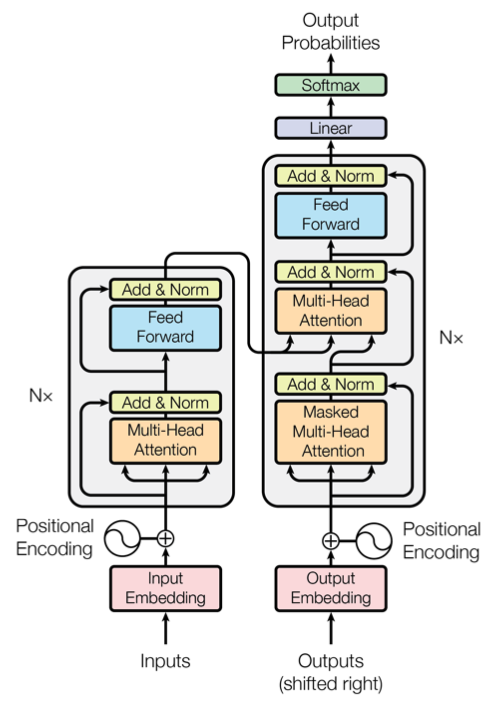
\includegraphics[width=0.4\textwidth]{Assets/transformers}
	\caption{\gls{Transformer} Architecture: Encoder and Decoder}
	\label{fig:transformers}
\end{figure}

For encoding text, only the Encoder part of the \gls{Transformer} is needed.
For generating text, the Decoder part is also needed (Fig.\ref{fig:transformers}).

\subsubsection{Self-Attention}
The central element in the architecture of \glspl{Transformer} is the \emph{self-attention mechanism} in the Multi-Head-Attention module depicted in Fig.\ref{fig:attn1}.

\begin{figure}[H]
	\centering
	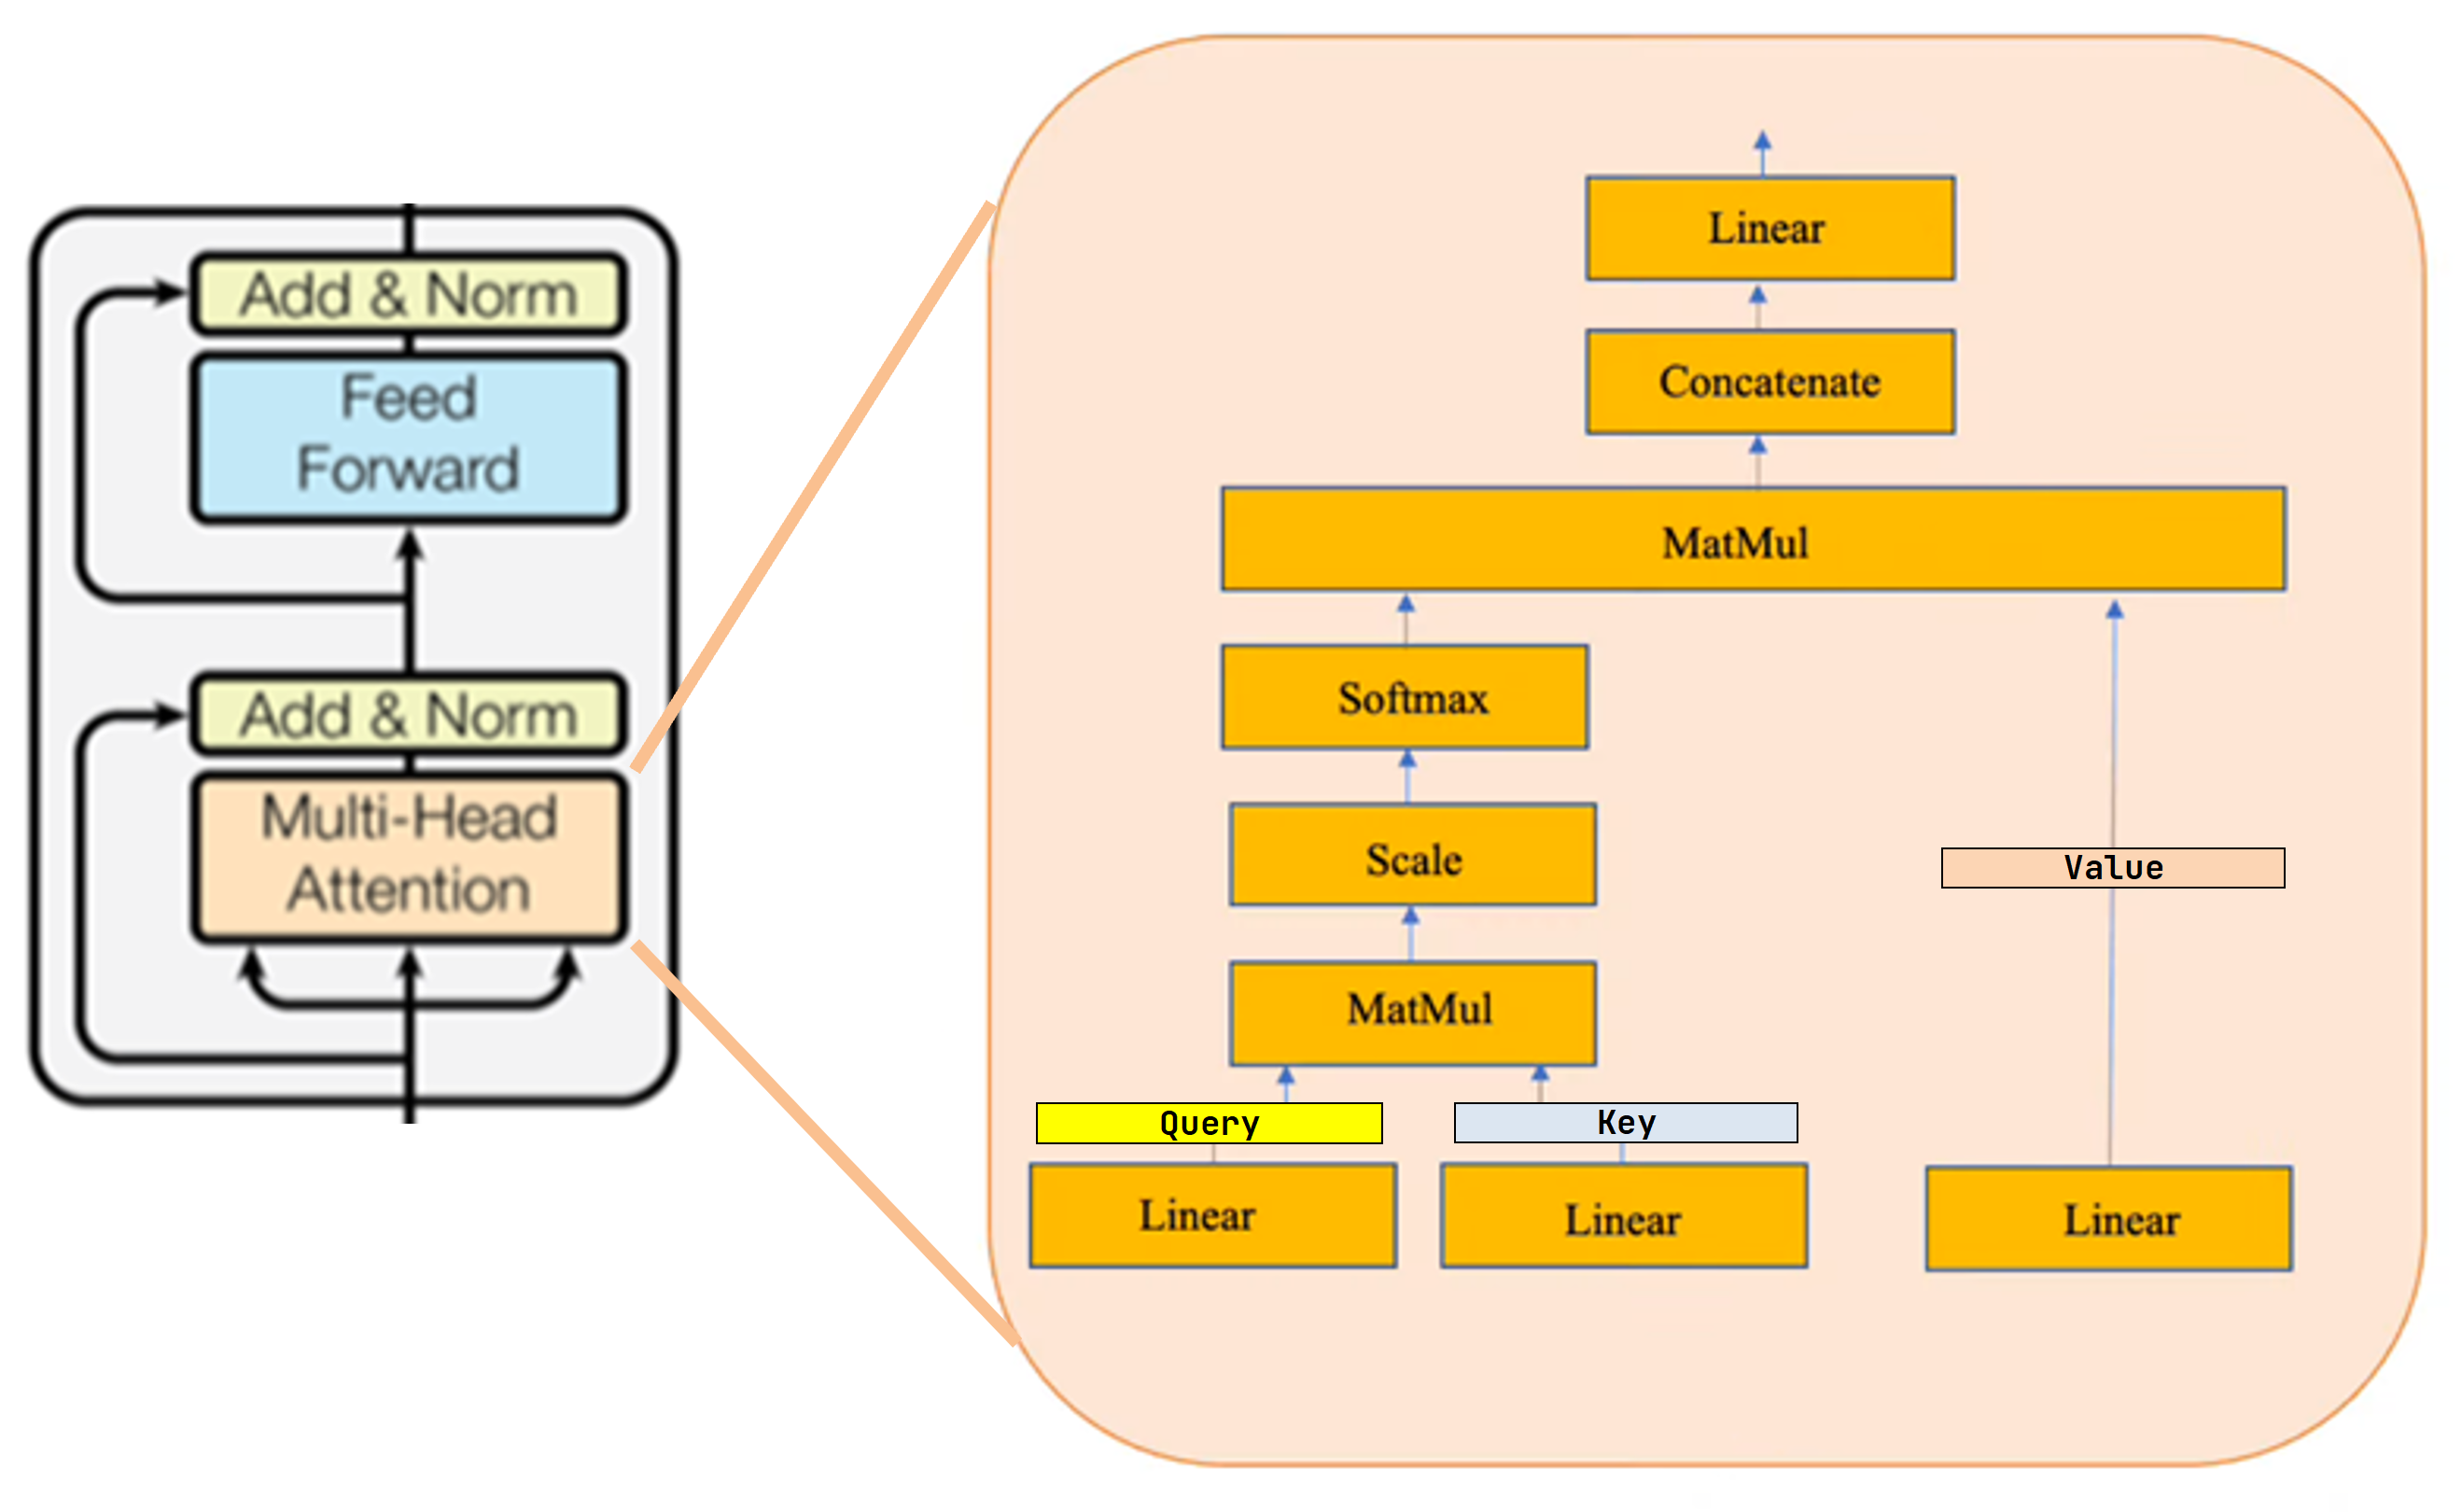
\includegraphics[width=0.7\textwidth]{Assets/attn1}
	\caption{Multi-Head Attention. Image from: \cite{BERT} and \cite{transformersyoutube}}
	\label{fig:attn1}
\end{figure}

In the Multi-Head-Attention module, three different matrices named \colorbox{yellow}{\emph{Query}}, \colorbox{cyan}{\emph{Key}} and \colorbox{orange}{\emph{Value}} are learned in the training phase based on one and the same static embeddings of the input words (Fig.\ref{fig:qkv1}).

\begin{figure}[H]
	\centering
	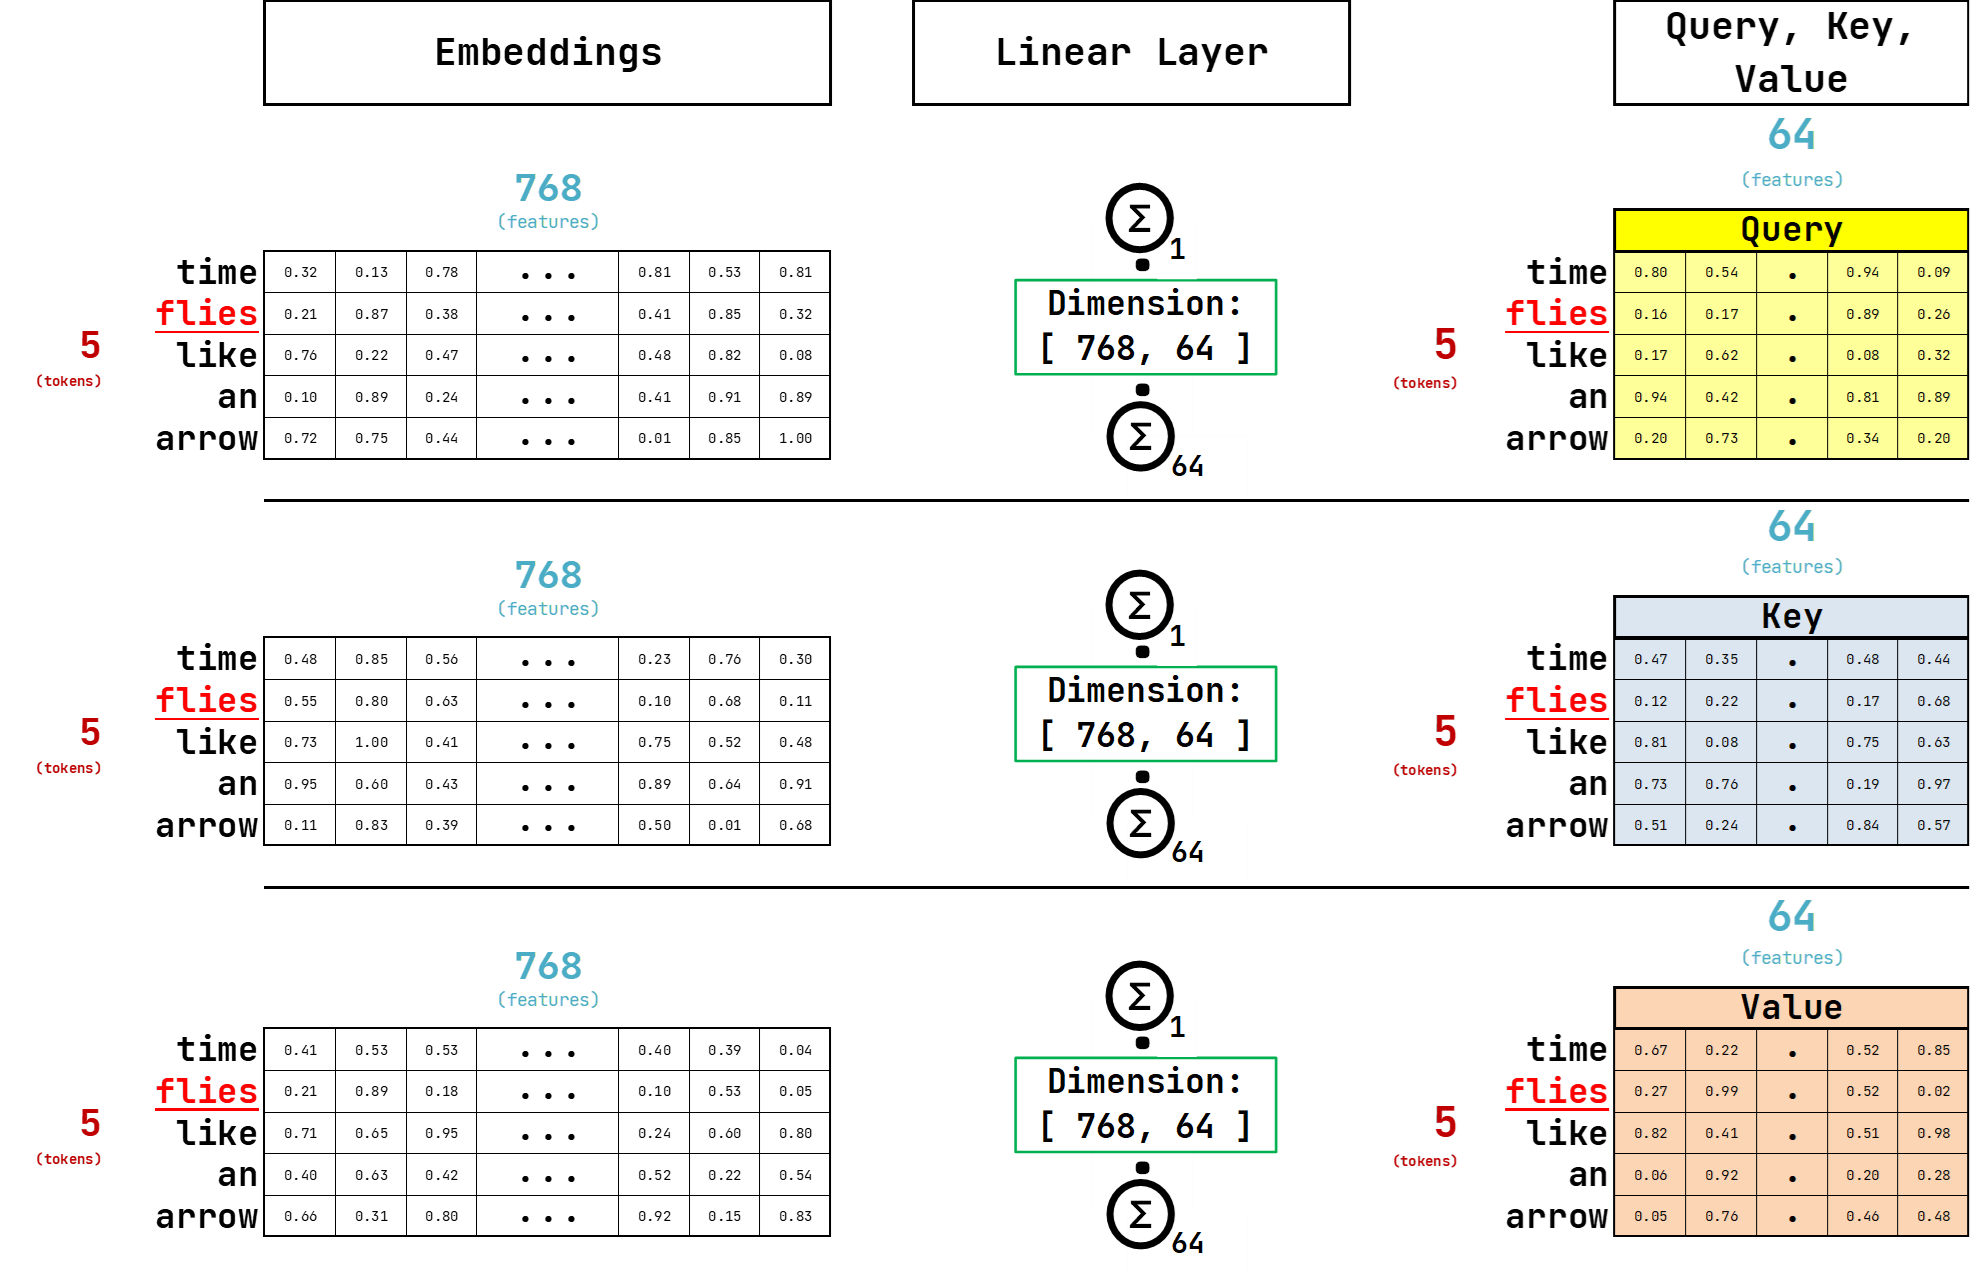
\includegraphics[width=0.7\textwidth]{Assets/qkv1}
	\caption{$Input Embeddings \cdot Linear Layer$ = \colorbox{yellow}{\emph{Query}}, \colorbox{cyan}{\emph{Key}}, \colorbox{orange}{\emph{Value}}}
	\label{fig:qkv1}
\end{figure}

The next step in the \emph{Multi-Head Attention} module during both, training and inference (in a downstream task), is the matrix multiplication depicted in Fig.\ref{fig:attnfilter} to produce the \colorbox{lime}{\emph{Attention Filter}}.
It has the same dimension ([5, 5] for the given sentence) as the length of the input text.
\begin{figure}[H]
	\centering
	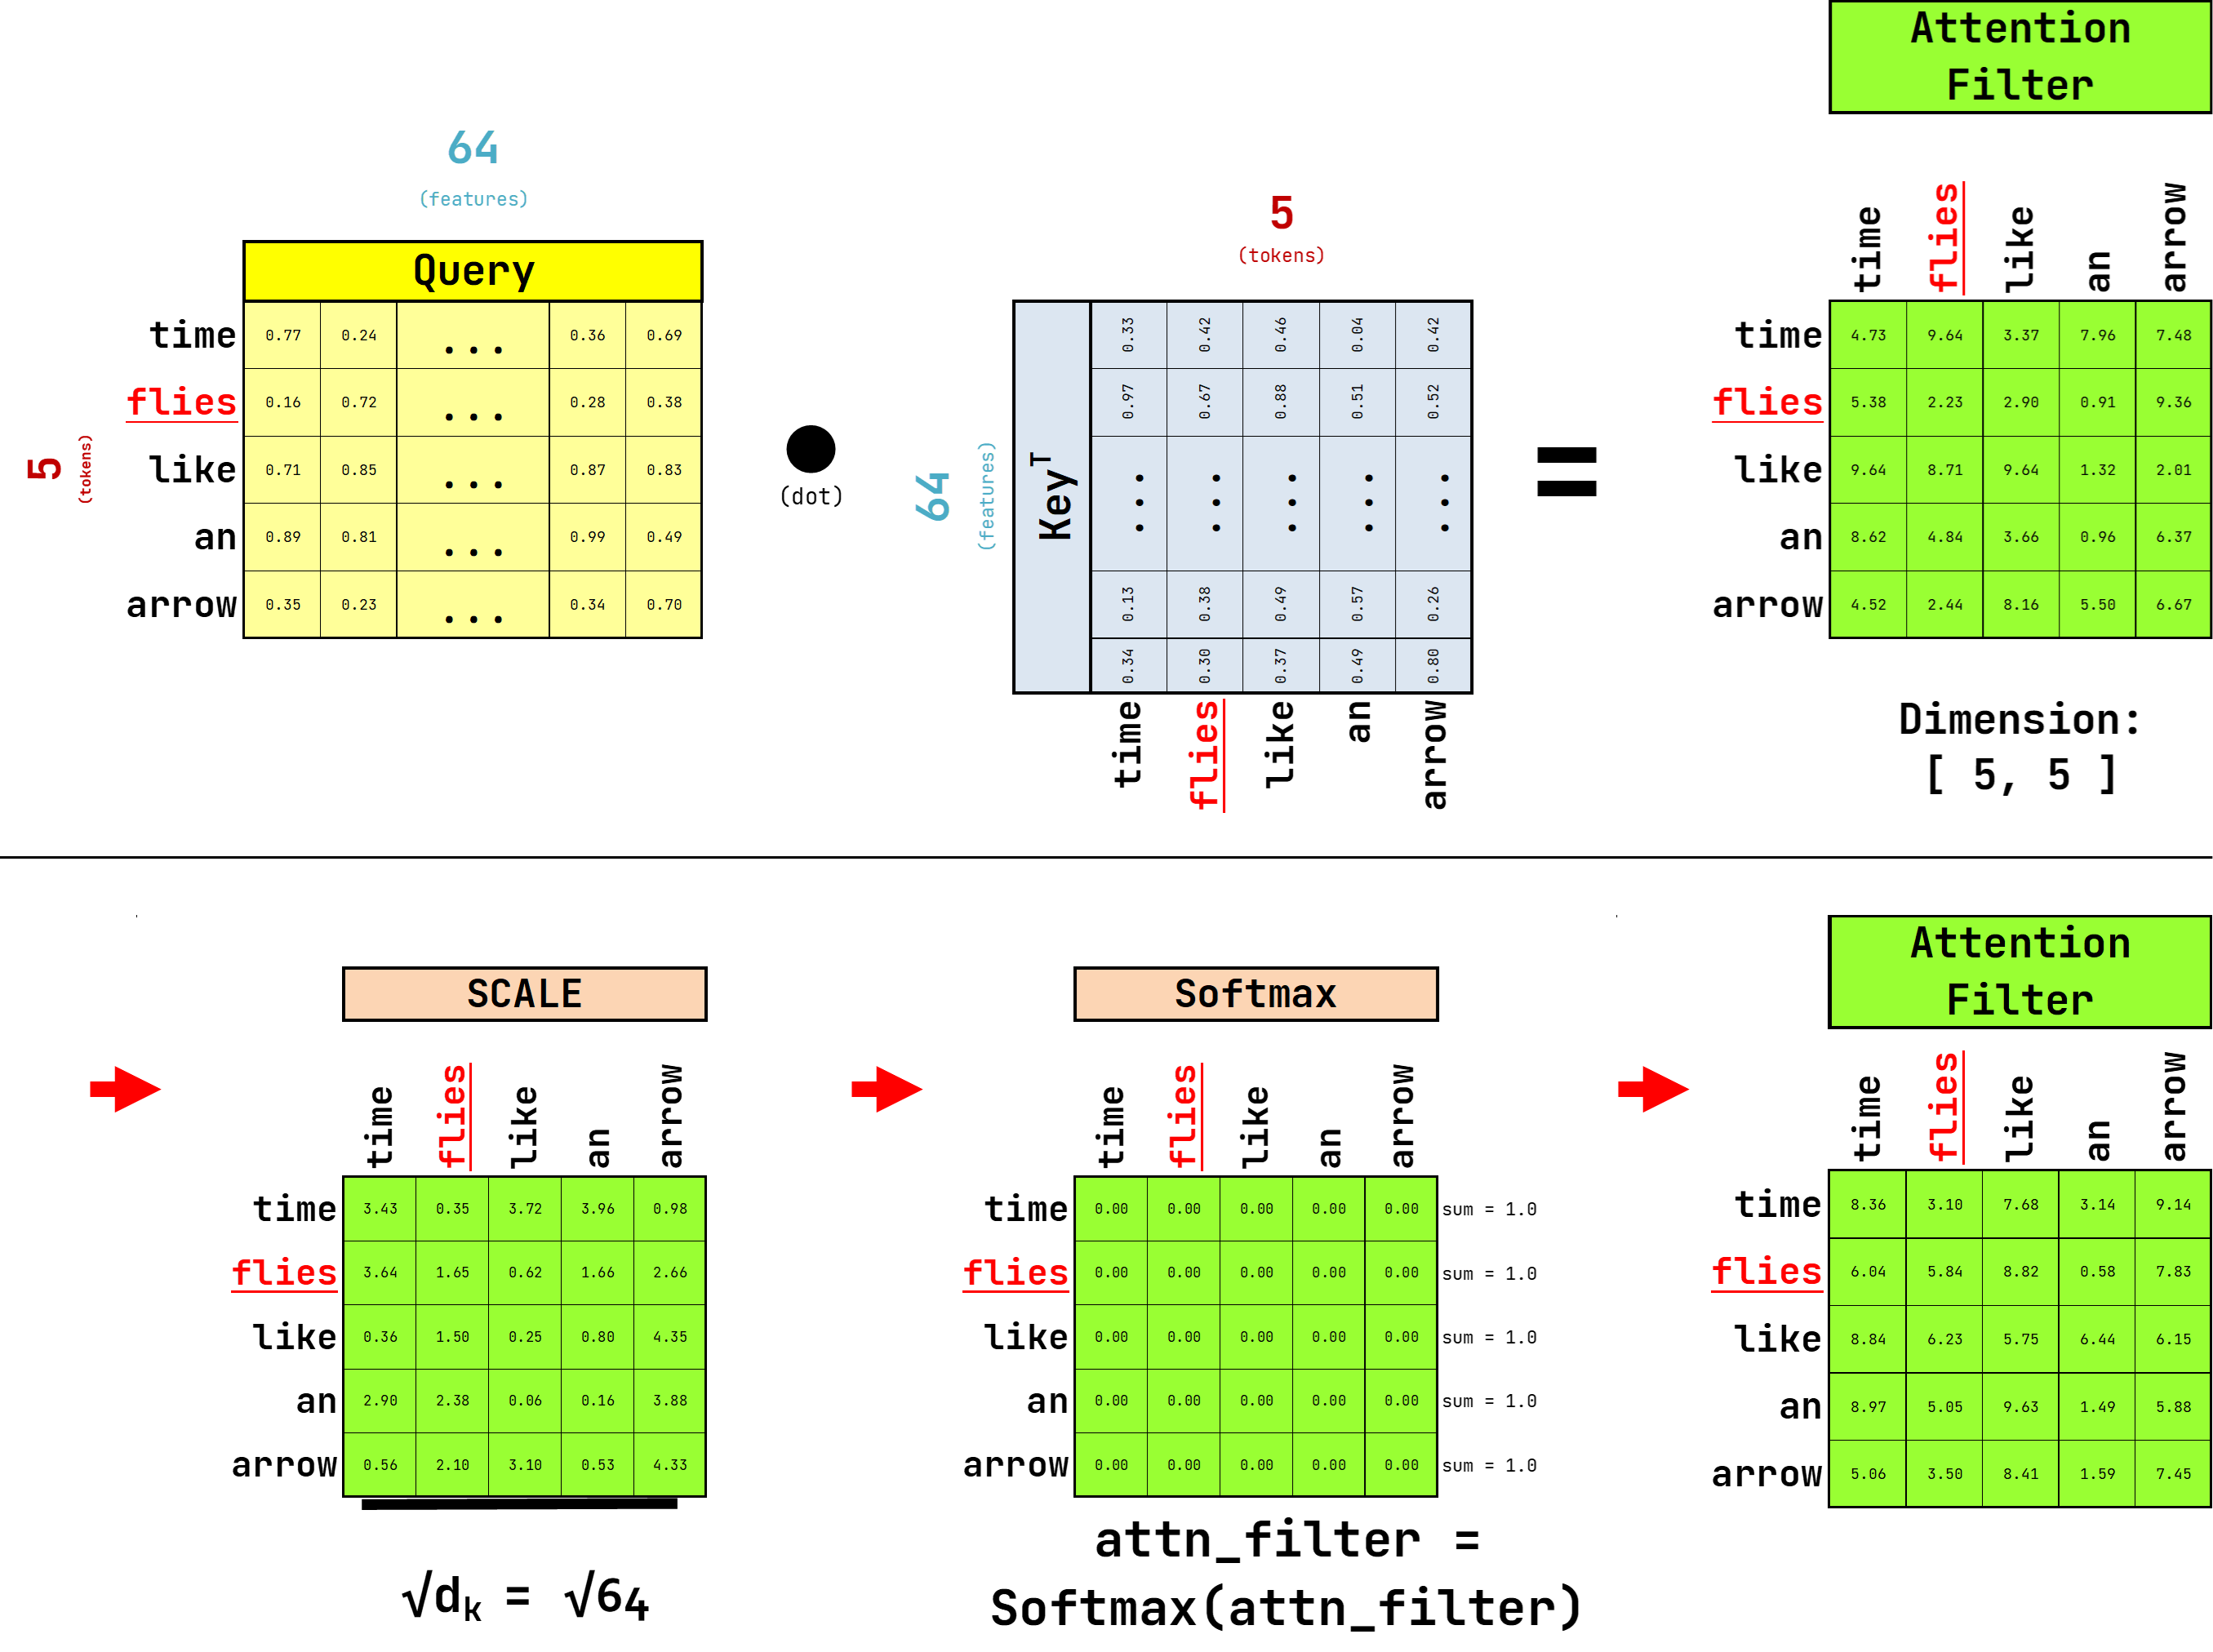
\includegraphics[width=0.7\textwidth]{Assets/attnfilter}
	\caption{$\colorbox{yellow}{\emph{Query}} \cdot \colorbox{cyan}{\emph{Key}}$ = \colorbox{lime}{\emph{Attention Filter}}}
	\label{fig:attnfilter}
\end{figure}

The task of the \colorbox{lime}{\emph{Attention Filter}} is to identify those adjacent words in a sentence that help determine the context for and
the meaning of a given word.

In the sample sentence \emph{time flies like an arrow}, a human reader would probably pay attention to the words \emph{arrow} and \emph{time} to determine the context and the meaning of the word \emph{flies}.
A well-trained \colorbox{lime}{\emph{Attention Filter}} would thus probably have higher values at the coordinate crossing for the word \emph{flies} (2nd row), \emph{time} (1st column) and \emph{arrow} (5th column).

The next step in the calculation process during training and inference is the most important and the main reason why \glspl{Transformer} can embedd context:
The multiplication of the \colorbox{lime}{\emph{Attention Filter}} with the \colorbox{orange}{\emph{Value}} matrix.

\begin{figure}[H]
	\centering
	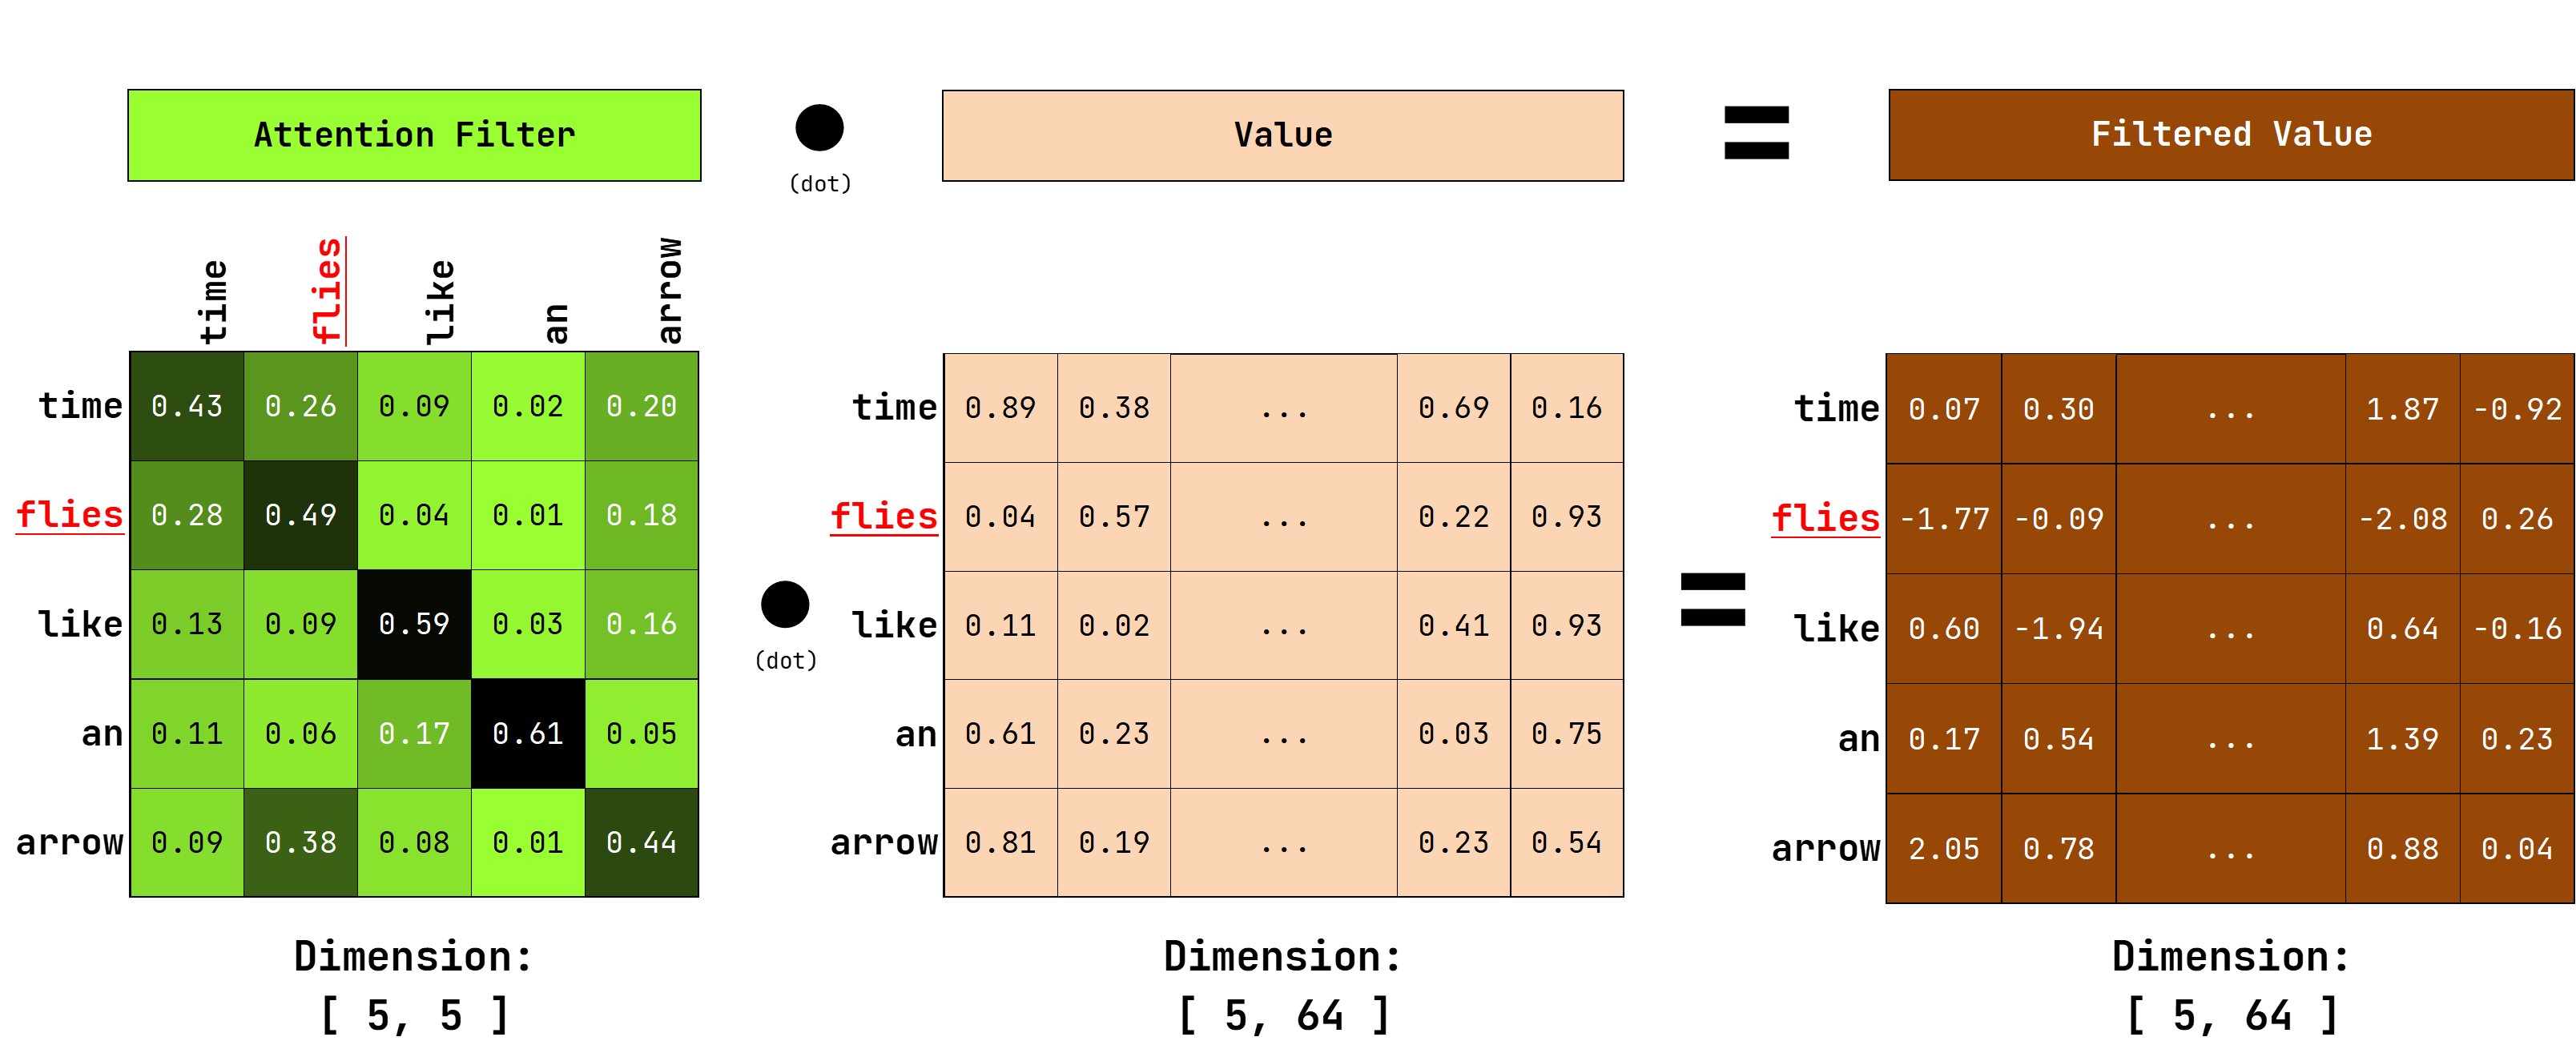
\includegraphics[width=0.7\textwidth]{Assets/filter1}
	\caption{$\colorbox{lime}{\emph{Attention Filter}} \cdot \colorbox{orange}{\emph{Value}}$ = \colorbox{brown}{\emph{Filtered Value}}}
	\label{filter1}
\end{figure}

The \colorbox{orange}{\emph{Value}} matrix is assumed to contain encoded information about the syntax and semantics of the input text though still static at this stage.
The \colorbox{lime}{\emph{Attention Filter}} multiplies the \colorbox{orange}{\emph{Value}} matrix carrying over those values to the \colorbox{brown}{\emph{Filtered Value}} matrix that are important to understand the context of the words.
As the \colorbox{lime}{\emph{Attention Filter}} is different for every sentence depending on its context, the resulting \colorbox{brown}{\emph{Filtered Value}} matrix contains the context-dependent embeddings.

To stress this important point, an example will be given that focuses on just one coordinate of the \colorbox{brown}{\emph{Filtered Value}} matrix: the 2nd row and the 1st column as shown in Fig.\ref{filteredvalues1}.

\paragraph{\emph{time flies like an arrow}}

\begin{figure}[H]
	\centering
	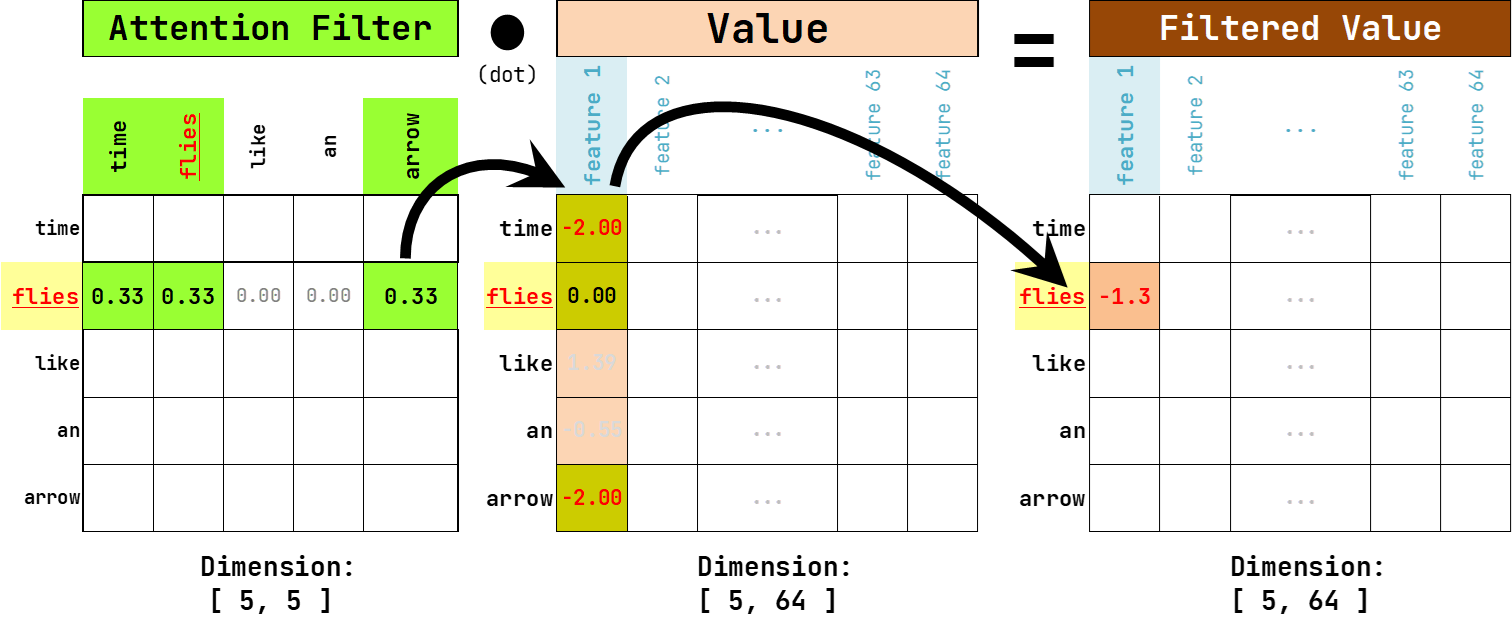
\includegraphics[width=0.9\textwidth]{Assets/filteredvalues1}
	\caption{\colorbox{brown}{\emph{Filtered Value}}: \emph{time flies like an arrow}}
	\label{filteredvalues1}
\end{figure}

It is assumed that the \colorbox{lime}{\emph{Attention Filter}} has identified the words \emph{time} and \emph{arrow} to be important context words for the word \emph{flies} in the sentence \emph{time flies like an arrow}.
The \colorbox{lime}{\emph{Attention Filter}} thus shows exemplary values of \textbf{0.33} for each of these context words and the word \emph{flies} itself, and a value of \textbf{0.00} for the remaining words \emph{like} and \emph{an}.

It is further assumed that the first column of the \colorbox{orange}{\emph{Value}} matrix represents a semantically interpretable feature that humans would describe as \emph{food-like} (like the column \emph{food} in the handcrafted feature table in Fig.\ref{fig:wordfeaturesmanually}).
If a given word in a wider sense has something to do with \emph{food}, it is assumed that the values in the first column of the \colorbox{orange}{\emph{Value}} matrix are positive, else zero or negative.
In Fig.\ref{filteredvalues1}, the exemplary \emph{food} feature values for the word \emph{time} and \emph{arrow} are \textbf{-2.00} as both words are assumed to have nothing to do with \emph{food}.
The exemplary \emph{food} feature value for the word \emph{flies} itself is assumed to be \textbf{0.00} (as some \emph{flies} might be edible insects and to make the point clearer).
The dot product of the 2nd row of the \colorbox{lime}{\emph{Attention Filter}} with the 1st column of the \colorbox{orange}{\emph{Value}} matrix so yields a value of \textbf{-1.3} at the 2nd row and 1st column of the \colorbox{brown}{\emph{Filtered Value}} matrix (see Fig.\ref{filteredvalues1}).


The 2nd row of the \colorbox{brown}{\emph{Filtered Value}} matrix already represents the contextualized or dynamic word embedding vector of the word \emph{flies} in the sentence \emph{time flies like an arrow}.
Whereas the \emph{food} feature value in the \colorbox{orange}{\emph{Value}} matrix for the word \emph{flies} was \textbf{0.00}, this value at the same coordinate in the \colorbox{brown}{\emph{Filtered Value}} matrix has changed to \textbf{-1.3}.
This change in the vector representation of the word \emph{flies} can be \underline{entirely attributed} to the negative \emph{food} feature value contributions coming from the words \emph{time} and \emph{arrow} in the \colorbox{orange}{\emph{Value}} matrix.

\paragraph{\emph{fruit flies like a banana}}
The same analysis is now done for the sentence \emph{fruit flies like a banana} shown in Fig.\ref{fig:filteredvalues2}.

\begin{figure}[H]
	\centering
	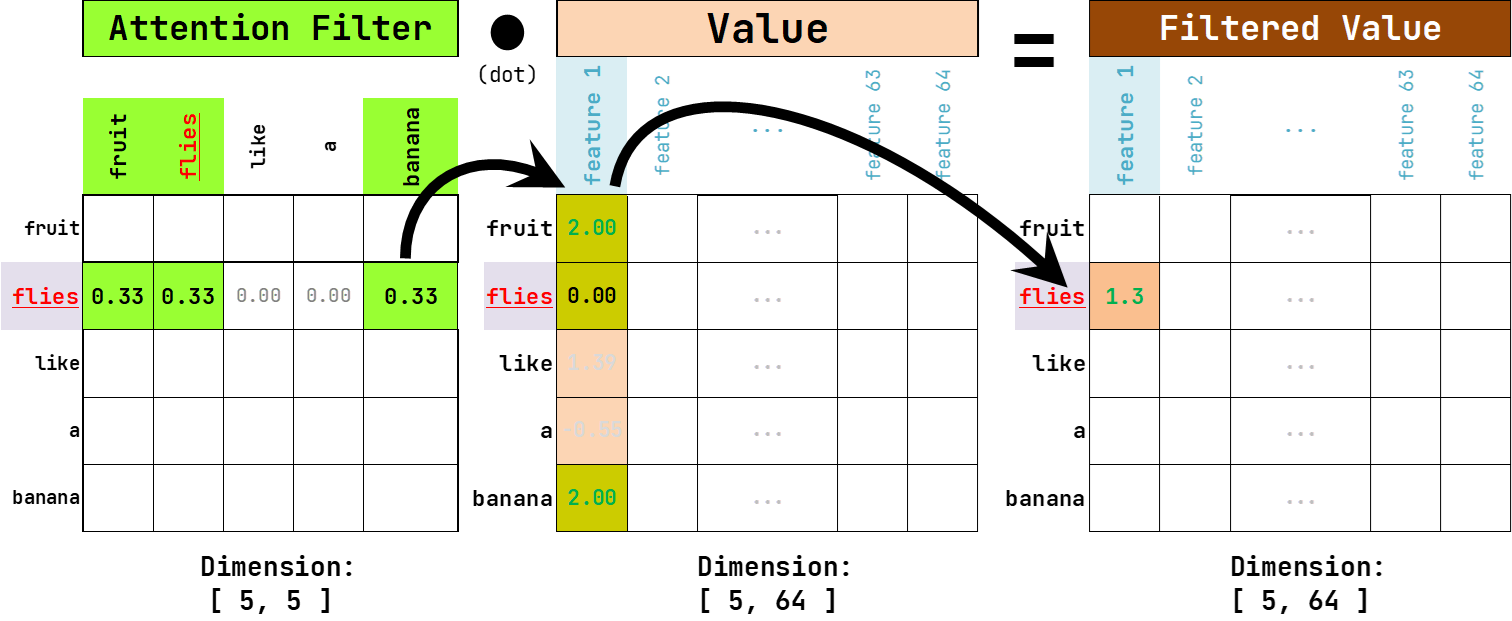
\includegraphics[width=0.9\textwidth]{Assets/filteredvalues2}
	\caption{\colorbox{brown}{\emph{Filtered Value}}: \emph{fruit flies like a banana}}
	\label{fig:filteredvalues2}
\end{figure}

Here, the assumption is that the \colorbox{lime}{\emph{Attention Filter}} has identified the words \emph{fruit} and \emph{banana} to be important context words for the word \emph{flies}, assigning the same exemplary values of \textbf{0.33} to them, like before.
The exemplary \emph{food} feature values for the word \emph{fruit} and \emph{banana} are now assumed to be \textbf{+2.00} as both words are strongly related to the idea of \emph{food}.
The exemplary \emph{food} feature value for the word \emph{flies} itself has not changed as it is indirectly coming from the static \emph{Input Embeddings}.
Every unique word (representation) in the \colorbox{orange}{\emph{Value}} matrix is the same for all sentences.
The dot product of the 2nd row of the \colorbox{lime}{\emph{Attention Filter}} with the 1st column of the \colorbox{orange}{\emph{Value}} matrix \textbf{now} yields a positive value of \textbf{+1.3} (see Fig.\ref{fig:filteredvalues2}), again coming from a value of \textbf{0.00} in the \colorbox{orange}{\emph{Value}} matrix.
This change in the vector representation of the word \emph{flies} in the \colorbox{brown}{\emph{Filtered Value}} matrix can be \underline{entirely attributed} to the positive \emph{food} feature value contributions coming from the words \emph{fruit} and \emph{banana} in the \colorbox{orange}{\emph{Value}} matrix.

\paragraph{\emph{Different embeddings for same word depending on context}}
The application of this principle to not only one column (here the \emph{food} feature column), but to all 64 columns of the \colorbox{orange}{\emph{Value}} and \colorbox{brown}{\emph{Filtered Value}} matrices, ensures that different semantic and syntactic aspects of word inter-dependencies are accounted for.
The \colorbox{brown}{\emph{Filtered Value}} matrix is where all the attention magic plays out.
Whereas the \colorbox{orange}{\emph{Value}} matrix can be considered a \textbf{static} word embedding, the \colorbox{brown}{\emph{Filtered Value}} matrix truly is a \textbf{dynamic} representation of words as it depends on the context words that are identified by the \colorbox{lime}{\emph{Attention Filter}} and that are different for every sentence.
The embedding vector of the word \emph{flies} in the \colorbox{brown}{\emph{Filtered Value}} matrix is different for the two sentences because the adjacent words to \emph{flies} are different and so is its context.\\
This means that \gls{Transformer}-based models can encode human language semantics and syntax much better than previous models.

%%%%%% Hallucination

\section{Is a \gls{gen-llm} all you need?}\label{sec:is-a-generative-llm-all-you-need?}
\paragraph{\glspl{gen-llm}}

A recent trend in \gls{nlp} seems to be the increasing use of \glspl{gen-llm}, like OpenAI's GPT models, for all kinds of \gls{nlp}-related tasks such as \gls{ner} or \gls{coref_resolution_definition}.
Instead of developing, pretraining or fine-tuning custom models using traditional programming languages, algorithms and datasets, researchers and practitioners seem to increasingly focus on engineering \glspl{prompt} to let \glspl{gen-llm} perform the task.

\paragraph{\gls{RAG} Systems}\label{par:rag-systems}
\gls{RAG} systems are sometimes added to such \glspl{gen-llm} in order to improve their accuracy.
\gls{RAG} stands for \emph{Retrieval Augmented Generation} and is a means to enrich a \gls{prompt} with relevant information.
Proprietary documents are typically chunked and loaded into a vector database to add context and information to the \gls{prompt}.
\gls{RAG} systems typically rely on vector similarity measures such as cosine similarity (see Section \ref{subsec:document-similarities}).
The text of a user question is converted to an embedding vector for which a similar embedding vector is searched in the vector database.
The text document with the highest cosine similarity is processed and formulated as an answer to the user's question.

\paragraph{The Hallucination problem}\label{par:hallucination}
Although \glspl{llm}, with contextual word embeddings at its core, have revolutionized the \gls{nlp}-world,
\gls{Hallucination}, or the presentation of false or misleading information as facts \cite{Hallucination}, still remains a problem and for some researchers is even inevitable \cite{hallucinationinevitable}.


\glspl{Hallucination} are often caused by the conflict between the user's intent and the characteristics of \glspl{llm}:

\begin{itemize}
\item Good \glspl{llm}, and good Machine Learning models in general, are supposed to \emph{generalize} well but are not supposed to \emph{memorize} their training data
\item \glspl{gen-llm} generate their text based on the highest probability for the next word
\item These probabilities hinge on the data fed to the \gls{llm} during training or retrieved from \gls{RAG}-systems
\end{itemize}

Generalization means that the \gls{llm} outputs text that fits learned patterns, but does not output the training (or \gls{RAG}) text itself.
Even if the training data was all true and factual (which is unlikely), the generated output text would most likely be different.
Even if a certain, factually correct text was part of the training data, an \gls{llm} ChatBot will most likely not return the same text.
Next word generation based on probabilities means, that of all candidate words the one word with the highest probability is taken, even if that probability itself is very low.

For a creative goal such as writing novels or poetry, this might not be a problem and often is a desired characteristic.
For the goal of retrieving or generating text that contains correct and accurate facts, this might be damaging as demonstrated by the \emph{ChatGPT-Lawyer}-case \cite{WebsiteChatGPTLawyer}, where a lawyer cited fake legal cases that were generated by ChatGPT.

Domain-specific training data and \gls{RAG}-systems can decrease \gls{Hallucination} rates, but not entirely.
A recent study \cite{hallucinationlegal} by Yale and Stanford researchers revealed that even domain-specifically trained, \glspl{gen-llm}
with extensive \gls{RAG}-systems attached to them, showed \gls{Hallucination}-rates of between 17 and 33 percent.

\paragraph{Questions in regard to LLMs}
Two of the questions for this project are driven by this problem.
The first question is:
\begin{center}
	\emph{Given the problem of hallucinations, how do \glspl{gen-llm} perform versus tradional methods on the task of information extraction?}
\end{center}
In the \emph{Information Extraction Pipeline}, different approaches will be studied, implemented in code and compared with each other.
This covers traditional rule-based and pre-trained \gls{ann} models, but also models based on \glspl{gen-llm}.\\

In the Knowledge Graph part, a ChatBot (\gls{graph-bot}) will be attached to the Knowledge Graph.
This is to elaborate on the question
\begin{center}
	\emph{Can Knowledge Graphs be used as an alternative to traditional RAG-systems?}
\end{center}
A recent research by Microsoft \cite{graphrag} does point in this direction, but does this also apply to this project and its data?\\

In the next chapter, the project and \emph{Information Extraction Pipeline} will start with extracting named entities.




